\documentclass[conference]{IEEEtran}
\IEEEoverridecommandlockouts
% The preceding line is only needed to identify funding in the first footnote. If that is unneeded, please comment it out.
\usepackage{listings}
\usepackage{wrapfig}
\usepackage{units}
\usepackage{cite}
\usepackage{amsmath,amssymb,amsfonts}
\usepackage{algorithmic}
\usepackage{graphicx}
\usepackage{textcomp}
\usepackage{xcolor}
\usepackage{float}
\usepackage{caption}
\usepackage{tocloft}
\usepackage{lipsum}
\usepackage{titlesec}
\usepackage{pdfpages}
\usepackage{xcolor}
\usepackage{colortbl}
\usepackage{siunitx}
\usepackage{physics}
\usepackage{tikz}
\usepackage{mathdots}
\usepackage{yhmath}
\usepackage{cancel}
\usepackage{color}
\usepackage{array}
\usepackage{multirow}
\usepackage{gensymb}
\usepackage{tabularx}
\usepackage{extarrows}
\usepackage{booktabs}
\usetikzlibrary{fadings}
\usetikzlibrary{patterns}
\usetikzlibrary{shadows.blur}
\usetikzlibrary{shapes}
\usepackage{hyperref}
\hypersetup{
colorlinks=true,
linkcolor=black,
filecolor=black,      
urlcolor=black,
citecolor=black,
}
\pagenumbering{Roman}
\renewcommand\thesection{\arabic{section}}
\renewcommand\thesubsection{\thesection.\arabic{subsection}}
\renewcommand\thesubsubsection{\thesubsection.\arabic{subsubsection}}
\def\BibTeX{{\rm B\kern-.05em{\sc i\kern-.025em b}\kern-.08em
    T\kern-.1667em\lower.7ex\hbox{E}\kern-.125emX}}
\titleformat{\subsection}
  {\bfseries \Large}{\thesubsection}{1em}{}

\setlength{\parindent}{.5 in}

\renewcommand{\contentsname}{\LARGE \begin{center}\textbf{Table of Contents}\end{center}\vspace{-15pt}}
\renewcommand{\listtablename}{\LARGE \begin{center}\textbf{List of Tables}\end{center}\vspace{-15pt}}
\renewcommand{\listfigurename}{\LARGE \begin{center}\textbf{List of Figures}\end{center}\vspace{-15pt}}

\let\LaTeXStandardTableOfContents\tableofcontents

\renewcommand{\cftsecleader}{\cftdotfill{\cftdotsep}}

\renewcommand{\cftsecfont}{\mdseries}
\renewcommand{\cftsecpagefont}{\mdseries}

\setcounter{section}{1}

\setlength\cftsubsecnumwidth{4em}
\setlength\cftsubsubsecnumwidth{5em}

\def\bibname{\LARGE References}\let\refname\bibname

\begin{document}

\title{\centering 
\includegraphics[height=.11\textheight]{Figures/NEU.png}\\ \vspace{15pt} \textbf{Encryption: An Educational Exhibit}\\ \vspace{5pt}\large \textbf{Cornerstone of Engineering — Fall 2022, 13767}\\ \vspace{15pt} \centering 
\includegraphics[height=.4\textheight]{Figures/Encrypted.png}\\ \vspace{15pt} \textsc{Submitted By}:\\ \vspace{10pt} \centering 
\includegraphics[height=.125\textheight]{Figures/goblin.jpg} \\ \vspace{15pt} \textsc{Prepared By}:} \thispagestyle{empty}

\author{\IEEEauthorblockN{Henry Shields}
\IEEEauthorblockA{\textit{Northeastern University} \\
\textit{Computer Science \& Eng.}\\
\href{mailto:Shields.H@Northeastern.edu}{Shields.H@Northeastern.edu}}
\and
\IEEEauthorblockN{Michael Brodskiy}
\IEEEauthorblockA{\textit{Northeastern University} \\
\textit{Physics \& Electrical Eng.}\\
\href{mailto:Brodskiy.M@Northeastern.edu}{Brodskiy.M@Northeastern.edu}}
\and
\IEEEauthorblockN{Michael Levy}
\IEEEauthorblockA{\textit{Northeastern University} \\
\textit{Undecided}\\
\href{mailto:Levy.Mi@Northeastern.edu}{Levy.Mi@Northeastern.edu}}
\and
\IEEEauthorblockN{Neil Dungca}
\IEEEauthorblockA{\textit{Northeastern University} \\
\textit{Chemical Eng.}\\
\href{mailto:Dungca.N@Northeastern.edu}{Dungca.N@Northeastern.edu}}
\and
\textsc{Report Submitted}: December 5, 2022
}

\maketitle

\onecolumn

\thispagestyle{plain}

\addcontentsline{toc}{section}{ABSTRACT}

\begin{center}
\LARGE \textbf{ABSTRACT}
\end{center}
\begin{justify}
\par This document outlines the decision making and analysis process, a meaningful engineering design process, and the data collection and review related to the fabrication of an educational exhibit intended for young adults.
\par The educational exhibit project, most importantly, was constrained by the theme ``espionage technology''. The project was also constrained by the following factors: safety during transportation and use, ease of transport, inclusion of at least two interactive elements, integration of at least two SparkFun components, and a total cost of less than \$100. In terms of objectives, the exhibit had to be: set up and broken down easily, engaging and educational for middle and high school students, able to handle regular interaction, and able to collect user data. In terms of design goals, the group focused mainly on education and accessibility in both our interactive and educational elements. 
\par To develop the most viable solution, a set of design goals were identified. These, from most to least important, determined that it was most important for the solution to be: educational, intuitive, interactive, accessible, and lightweight. Given these goals, the solution was accepted to be an encryption-decryption game, due to its highly educational and interactive nature. Such a solution would involve two players: one entering a phrase to be encrypted\footnote{The encryption would be fairly simple, with an ASCII character shift of a randomly-generated value (to make the decryption easily guessable in a short time)}, and setting a certain time frame for the other player to guess. On a second display, the second player is first told how many characters the letters have been shifted by, and, using a provided table, determines the original phrase, hopefully within the time frame. Once the round is over, the players are asked to switch sides, so both players get to experience both sides. The program records player names, ages, entered phrase, post-encryption phrase, and the time to correctly decrypt (if within the allotted time).
\par The design functioned quite well, as the level of engagement was fairly high. This is indicated by the fact that, at almost all times, there was a queue to play, even though the time limits per round were set to be fairly short (30-60 seconds). The biggest downfall seemed to be that, even with the exact ASCII-shift value given to the decrypting player, the game was still quite difficult, as indicated by the fairly low win rate (43.75\%). As such, the design functioned entirely as intended, but may have been difficult for students at a middle or high school level.
\end{justify}

\addcontentsline{toc}{section}{KEYWORDS}

\begin{center}
\LARGE \textbf{KEYWORDS}\\
\end{center}
\begin{justify}
  \underline{decision analysis}, \underline{engineering design process}, \underline{espionage technology}, \underline{educational exhibit}, \underline{constraints}, \underline{objectives}, \underline{user data}, \underline{encryption}, \underline{decryption}, \underline{interactive}
\end{justify}

\newpage

\Large

\tableofcontents

\newpage

\addcontentsline{toc}{section}{LIST OF TABLES}

\Large

\listoftables

\addcontentsline{toc}{section}{LIST OF FIGURES}

\listoffigures

\twocolumn

\pagenumbering{arabic}

\newpage

\addcontentsline{toc}{section}{HENRY SHIELDS}

\vspace{10pt} \LARGE \textbf{HENRY SHIELDS} \normalsize

\subsection{Introduction}

\par This project aims to equally and indiscriminately educate students and children who will attend the first-year engineering annual project exhibition on The Technology of Spyware. The primary stakeholders are the students who will find inspiration, education, and interest in the information and design that is not typically displayed in a common core environment.  
\par The idea behind this exhibition is to generate excitement and interest in engineering via an unorthodox and entertaining approach. To do so, however, the project must be portable and easily set up with a minimal amount of people. Likewise, it must be able to deconstruct into the given parameters of the box provided. It also must be resilient enough to withstand numerous interactions with children and allow accessibility in all cases. To achieve this goal, the visual elements will be tiltable and the contrast adjustable to ensure any physical impairment will not interfere with the education. To promote essential engineering values such as teamwork, the design will be multiplayer and focus on working together to solve a problem. Furthermore, it is required that the design utilize both Arduino and MATLAB, with additional elements such as an LED timer and audio provisions for the visually challenged. 
\par To inspire interest and a deeper understanding of the complex technology present everywhere in the modern world, the students will be tasked with using materials and their peers to decipher a code. To maximize understanding they will essentially be unknowingly going through the same steps as the computer. As referenced in the research, many children simply accept technology as they were born into it, however, it is the aim of this project to foster a deeper kinship and passion for how that technology works. 
\par There are numerous restraints, however the most prevalent is pricing. This multiplayer encryption design utilizes expensive parts such as a laptop, LCD display, and a Bluetooth keyboard. Thus, most of the physical elements will be relied upon by free recycling bins such as those at FYELIC. The presentation must also be engaging and cooperative for all ages, seeing as the abilities of a high schooler compared to an elementary schooler are quite stark. The educational panels and instructions then must be easily skimmable if the user is familiar with the ideas that the project is based on, and if needed, in-depth for those who have no prior experience or knowledge. 

\subsubsection{Scope}

\par This technical report will serve to evaluate the full engineering design process of The Malignity of Goblins. It also includes user data collection, code, images of the construction, and circuits. 

\subsection{Background}

\par Since the days of WWII and the Cold War, spy technology has been prevalent in military and entertainment programs. The natural interest of the public in secretive measures, especially those that impact enemy countries is of utmost curiosity. As represented in films like the James Bond series or cartoons such as Spy vs Spy, the hidden technology of spyware has been widespread to the public. It is only natural then, that exhibits and museums such as the very one this project aims to create, have developed naturally over time. One such example is SciTech in Perth, Australia, which has a myriad of exhibits such as hidden cameras, phone taps, safe breakers, hidden bugs, and sound beams to name a few. This exhibit equips the visitor with a “Spy File” to gather information and utilize the scientific process along the way. It is within SciTech’s message to support STEM Education, and they believe this is accessible and accomplished for all. For educators and students, whom this is aimed at as well, they have lessons, essential questions, and debriefs. Another existing solution lies in the Spy Museum of Tampere, Finland. This museum is unique as it opens its doors to not just exhibits or museum-specific creations, but rather real spyware utilized from the First World War to the end of the Cold War. Some exhibits at this location include a bug detector, used in the 1930s and still operational, cipher machines, radio communications, an Enigma-E machine, and a NATO Toxic Suit. This museum is harder to replicate as it uses historic real spyware, however, the education and entertainment behind the science are still prevalent. There are set-up scenes of World War information offices, tests for kids, such as one to become the next 007, and a fake recommendation to an important international agency. This test educates the user while collecting information. To create a successful design, research was done into these existing solutions to pull inspiration such as this data collection or examples of devices and how they work. 
\par Furthermore, educational research was conducted to teach students while retaining their attention and entertainment effectively and efficiently. A few tips recommended by greater industry sources found in the research are as follows. First, to ensure the design is unique as to copy or create something unoriginal is the easiest way to lose the attention and respect of the client and user. Secondly, while focused on engineering and technology, this project is an exhibit, and an exhibit is meant to be creative, thus, emphasis is crucial. The project should be an experience, not a lecture, and thus the layout and design should use as many senses as possible. In the spirit of this advice, the last tip is to avoid overloading the user. There should be a good amount of information present, but not so much that there is no room for design, entertainment, and the formulation of the user’s own imagination. This is crucial seeing as our target audience is the young and impressionable engineers of tomorrow. 
\par The definition of success is a design that captures the attention, gets across the point, and leaves the user with a sense of wonder and understanding. By researching prior designs as well as educational methods, the project will have the needed inspiration, passion, and real comprehension as to how best to educate the students.  

\subsection{Methodology}

\subsubsection{Developing the Problem}

\par To create this design, The Malignity of Goblins participated in a full and thorough evaluation of the engineering design process. Firstly, background research was performed in each member’s separate efforts, and each wrote a short summary of the important discoveries, takeaways, and lessons, from the research. This was mainly broken into two categories, edutainment, which is a term to describe the combination of learning while also interacting and enjoying an exhibit, and spyware specifics. Then, the information was combined into one cohesive review, and evaluations were made on individual technologies, organizations that host spyware exhibits, and how best to use our knowledge in education and artistic display to create a better final product. Using all that was gained from research, a problem statement dictating the constraints, objectives, and stakeholders was created. 

\subsubsection{Generating the Solution}

\par This leads to the second section of the design process, generating solutions. Each member of the group created two unique designs separate from the rest of the members and then the sketches and explanations were shared between us. From here it went to brainstorming, gallery displays, and somewhat random association to create a series of unique ideas. 

\subsubsection{Decision-Making}

\par Thirdly, an idea had to be selected in a quantitative and accurate manner. To do so, we rank-ordered five criteria: educational, interactive, accessible, intuitive, and lightweight. After comparing the rankings against each of the criteria, objective weightings were created as follows: educational - 100, intuitive - 80, interactive - 70, accessible - 50, and lightweight - 20. By multiplying each design ranking out of ten in each category by the weighted numbers given above, everyone summed each row to create quantitative comparisons. The four separate charts and weighted results were then averaged and composed into one group KTDA. The seven designs were compared with the highest result being the multiplayer encryption game with an average result of 2265. 

\subsubsection{Implementation}

\par The fourth, and largest step, was implementation. This step was by far the lengthiest and required managing money, time, and all other resources. To do so, every week a Gaant chart and updated bill of materials were created to track both time-sensitive goals and individual tasks, as well as the funds left for the project as the specifications require the cost to be under \$100. To start implementing the idea into reality, firstly a SolidWorks sketch was designed to display the design in three dimensions in both “closed” form, that is when the contraption is collapsed to save space, and “open” form, that is when the device pops fully into standing position. Secondly, a proof of concept was designed which consisted of a cardboard pop-up Atari-appearing contraption and a MATLAB App that was able to take in a word and encrypt it, displaying back to the user. The decryption at this point consisted of the user typing in how many ASCII values the word had been rotated by, and if correct, a message would be displayed. After receiving feedback and reevaluating the design, some changes were made. Firstly, in physical conception, the design lost its pop-up feature and instead opted for a smaller two-part system with one side holding the LCD Monitor and the electronics, and the other holding the laptop that the MATLAB App would run on. The second change came in the form of MATLAB App code and design. The former of which was adjusted to have the user type in their guess and live display it to the LCD Display rather than type in an ASCII value off. This led to far more interaction and excitement. The program also displayed a range of ASCII values that the guess is off due to our results of testing being too difficult. The design was also changed simply for aesthetics to create neat and attractive buttons and text boxes. 

\subsubsection{Review \& Communication}

\par Finally, the last topic of review and technical/engineering communication. Throughout the entire process of developing the device, The Malignity of Goblins practiced professional reporting and communication via status memos, town hall presentations, and the recording of the design notebook. This ultimately climaxes in this very tech report, which is the culmination of all previous write-ups and memos, and the last piece of the engineering design process to learn from. 

\newpage

\addcontentsline{toc}{section}{MICHAEL BRODSKIY}

\vspace{10pt} \LARGE \textbf{MICHAEL BRODSKIY} \normalsize

\subsection{Introduction}

\subsubsection{Problem Statement} \label{ps}

\par This project serves to benefit the group of children that will be attending the showcase and learning about our project. The goal is to educate them all equally regardless of who they are and where they are coming from. The primary stakeholders are the children themselves as this showcase can provide them with information and inspiration they may not find in their regular schooling. Explicitly stating our engineering design process step by step helps us better understand the basic principles of our design.
\par The intention is to get students excited about the technology behind our design and encourage individual research. In terms of the physical presentation method, it must be easily set up and taken down by a minimal number of people. It also needs to be able to handle multiple interactions with, and be accessible for children, specifically those who are underprivileged and may not have prior STEM education. This means adjusting the interactive elements, such as tilting visual elements for kids in wheelchairs that see things on an upwards angle. Similarly, we want our interactive element to promote essential engineering values like teamwork. We also must make sure the individual parts fit inside the box given to us when deconstructed. Additionally, making sure we synthesize our ideas with the capabilities of the arduino and matlab is a necessity. We want  our design to include additional visual elements to the LCD screen like lights that time the user. 
\par Aside from the general education element of our project, the accessibility of the project and the emphasis on engineering values makes it important. The design will function in a way that maximizes understanding. A large part of the exhibition's aim is to show the kids how to utilize the resources they are given as well as collaborate with the people around them to accomplish a shared goal. As referenced in our research, a lot of children simply accept the complicated technology they use everyday without questioning how we as a society achieved that.
\par One of the largest constraints is going to be pricing. Our idea contains a lot of expensive elements and we are going to have to heavily rely on resources like FYELIC as well as modify our design if the materials are not available. Aside from just participation, the presentation must also be engaging and cooperative. Middle and high schoolers, on top of having very different interests, also comprehend topics differently. A student in high school is not going to need some of the basic information necessary for younger students. Because of this, there must be a greater emphasis on the presentation of information through interactive components of the design. We also want our project to be unique which, when basing it off of older technology, could be difficult. This means we really have to focus on the presentation of our information and work hard to customize our interactive elements.

\subsubsection{Stakeholders}

\par The main stakeholders involved in the project are the middle and high schoolers for which the educational exhibit is intended for; if the exhibit fails to educate this demographic, then it has failed in its main purpose. As such, this indicates that the primary stakeholders in the given situation are the children, as, in this case, they are the users, and, thus have the most to lose.
\par The client in the given scenario is Professor O'Connell and the College of Engineering. As they are the ones guiding the objectives of the projects, and setting the constraints. In this manner, they act as the secondary stakeholders, as, given failure, this would reflect negatively on them.

\subsubsection{Scope}

\par This report thoroughly covers the entire meaningful engineering design process in which The Malignity of Goblins engaged in.

\begin{figure}[H]
  \centering
  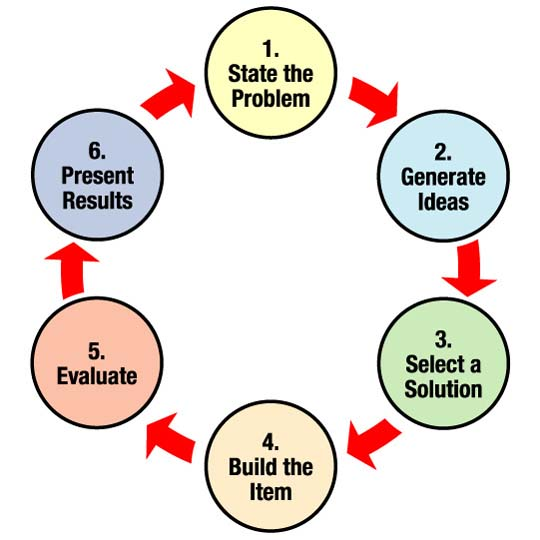
\includegraphics[width=.45\textwidth]{Figures/EDP.jpg}
  \caption{Full Engineering Design Process}
  \label{fig:1}
\end{figure}

\subsection{Background}

\subsubsection{Research}

\par Education is an ever-evolving aspect of everyday life. Every decision someone makes is based on the knowledge they attained at one point or another in their life; as such, it is important to expand one's horizons as much as possible. In this manner, the fabrication of an educational exhibit that covers topics which are generally not part of one's education is of utmost importance; furthermore, it is even more important to educate the coming generations, as the future of the world will soon rely on them. Thus, the central idea of this report is invariably relevant.
\par In researching germane exhibits, one of the most helpful resources was the list of exhibits at the International Spy Museum \cite{b7}. Going over the list of exhibits allowed the imagination to explore a deluge of possibilities; however, one of the most prominent issues with these exhibits was that they were not easily transportable — an important client-requested constraint. As such, though the essence of these exhibits was relevant, their viability in the given scenario was not very high, meaning that it was necessary to look elsewhere.
\par Continuing the research, it was necessary to look into relevant topics with which I was already familiar — one such topic was cryptography \cite{b4}. Delving into this topic, a simplified version of encryption (\textit{i}.\textit{e}.\ ASCII-shifting) seemed like a simple, accessible option for a game; on top of this, creating an encryption-based exhibit could allow us to discuss the history of the topic, and discuss the evolution of encryption-based technology, thereby also educating the children on the history of the topic.
\par With a viable option in mind, it was now time to research how best to implement it. Through research, it was found that exhibits which actually engage users allow for optimal learning \cite{b10}. In this manner, it was necessary to construct an interactive exhibit. One helpful source listed several tips on how to best create an interactive exhibit \cite{b11}. Taking notes from this source, it was decided that it would be best to create something simple, yet unique. Thus, it was settled that a two-player encrypt-decrypt game was the way to go.

\subsubsection{Ethics}

\par Given the evolution of technology, it is necessary to keep ethical considerations in mind. Most importantly, the exhibit needs to take safety of the user into consideration, especially given that primarily children will be interacting with it. Thus, during construction, the wood was sanded until fully smooth, and all circuitry was abstracted from the user.
\par Additionally, given the added functionality of data collection, as always, concerns of what data is collected exist. The program explicitly states which data is collected; it is also an option not to enter a name or an age.

\subsubsection{Universal Design}

\par As with any engineered contraption, it is necessary to take value sensitive design into account. In this manner, one of the group-defined objective goals to which we adhered to was accessibility. By making the game exhibit equally accessible to as many people as possible, we hoped to allow for a universal design, as outlined in \cite{b23}.

\subsection{Methodology}

\subsubsection{Defining the Problem}

\par First and foremost, the problem needed to be defined. As shown in \ref{ps}, a problem statement was generated in order to better synthesize the objectives, functions, constraints, and self-identified goals. Some of the most important objectives defined in the problem statement include, but are not limited to: conveying a sense of evolution and history of a piece of technology, keeping the user engaged while learning, and making interactivity a priority of the design. This way, it was simple to move to the next step, as the statement laid out a foundation for solution generation.

\subsubsection{Generating a Solution}

\par Given each team member's research, several possible solutions were identified. Using several methods, including, but not limited to, horizontal and lateral thinking, word association, and the SCAMPER method, the team was able to ideate meaningful designs.
\par The relevant designs generated were: stealth technology using a ball launcher or digitally, an encryption game, both single and multiplayer, a heel transmitter, an invisible ink game, and the detection of wire taps.
\par Figure \ref{fig:1} below identifies how the encryption game was initially supposed to work.

\begin{figure}[H]
  \centering
  \tikzset{every picture/.style={line width=0.75pt}} %set default line width to 0.75pt        

\begin{tikzpicture}[x=0.75pt,y=0.75pt,yscale=-.55,xscale=.55]
%uncomment if require: \path (0,582); %set diagram left start at 0, and has height of 582

%Shape: Ellipse [id:dp3892963566590173] 
\draw   (11,41.5) .. controls (11,21.34) and (38.31,5) .. (72,5) .. controls (105.69,5) and (133,21.34) .. (133,41.5) .. controls (133,61.66) and (105.69,78) .. (72,78) .. controls (38.31,78) and (11,61.66) .. (11,41.5) -- cycle ;
%Straight Lines [id:da19887855056316295] 
\draw    (72,78) -- (72,125.42) ;
\draw [shift={(72,127.42)}, rotate = 270] [color={rgb, 255:red, 0; green, 0; blue, 0 }  ][line width=0.75]    (10.93,-3.29) .. controls (6.95,-1.4) and (3.31,-0.3) .. (0,0) .. controls (3.31,0.3) and (6.95,1.4) .. (10.93,3.29)   ;
%Shape: Rectangle [id:dp014208133529669098] 
\draw   (11,128) -- (133,128) -- (133,201) -- (11,201) -- cycle ;
%Flowchart: Document [id:dp8688522724734018] 
\draw   (11,486) -- (133,486) -- (133,546.23) .. controls (56.75,546.23) and (72,567.94) .. (11,553.89) -- cycle ;
%Straight Lines [id:da5839938576291159] 
\draw    (72,200.42) -- (72,247.84) ;
\draw [shift={(72,249.84)}, rotate = 270] [color={rgb, 255:red, 0; green, 0; blue, 0 }  ][line width=0.75]    (10.93,-3.29) .. controls (6.95,-1.4) and (3.31,-0.3) .. (0,0) .. controls (3.31,0.3) and (6.95,1.4) .. (10.93,3.29)   ;
%Shape: Rectangle [id:dp912979444091131] 
\draw   (183,484) -- (305,484) -- (305,557) -- (183,557) -- cycle ;
%Straight Lines [id:da5083600057856885] 
\draw    (244,484.5) -- (244,437.08) ;
\draw [shift={(244,435.08)}, rotate = 90] [color={rgb, 255:red, 0; green, 0; blue, 0 }  ][line width=0.75]    (10.93,-3.29) .. controls (6.95,-1.4) and (3.31,-0.3) .. (0,0) .. controls (3.31,0.3) and (6.95,1.4) .. (10.93,3.29)   ;
%Straight Lines [id:da1366751880696635] 
\draw    (133,520.23) -- (180.42,520.23) ;
\draw [shift={(182.42,520.23)}, rotate = 180] [color={rgb, 255:red, 0; green, 0; blue, 0 }  ][line width=0.75]    (10.93,-3.29) .. controls (6.95,-1.4) and (3.31,-0.3) .. (0,0) .. controls (3.31,0.3) and (6.95,1.4) .. (10.93,3.29)   ;
%Shape: Rectangle [id:dp1281567774491723] 
\draw   (183,362) -- (305,362) -- (305,435) -- (183,435) -- cycle ;
%Shape: Boxed Line [id:dp041257977100174203] 
\draw    (305,399) -- (352.42,399) ;
\draw [shift={(354.42,399)}, rotate = 180] [color={rgb, 255:red, 0; green, 0; blue, 0 }  ][line width=0.75]    (10.93,-3.29) .. controls (6.95,-1.4) and (3.31,-0.3) .. (0,0) .. controls (3.31,0.3) and (6.95,1.4) .. (10.93,3.29)   ;
%Flowchart: Decision [id:dp6100652602081542] 
\draw   (415.42,362.5) -- (476.42,399) -- (415.42,435.5) -- (354.42,399) -- cycle ;
%Straight Lines [id:da2210516933251061] 
\draw    (415.42,362.5) -- (415.42,315.08) ;
\draw [shift={(415.42,313.08)}, rotate = 90] [color={rgb, 255:red, 0; green, 0; blue, 0 }  ][line width=0.75]    (10.93,-3.29) .. controls (6.95,-1.4) and (3.31,-0.3) .. (0,0) .. controls (3.31,0.3) and (6.95,1.4) .. (10.93,3.29)   ;
%Flowchart: Decision [id:dp5795837488593116] 
\draw   (415.42,241) -- (476.42,277.5) -- (415.42,314) -- (354.42,277.5) -- cycle ;
%Straight Lines [id:da8276046312641692] 
\draw    (415.42,240.5) -- (415.42,193.08) ;
\draw [shift={(415.42,191.08)}, rotate = 90] [color={rgb, 255:red, 0; green, 0; blue, 0 }  ][line width=0.75]    (10.93,-3.29) .. controls (6.95,-1.4) and (3.31,-0.3) .. (0,0) .. controls (3.31,0.3) and (6.95,1.4) .. (10.93,3.29)   ;
%Shape: Rectangle [id:dp40043316067990364] 
\draw   (355,119) -- (477,119) -- (477,192) -- (355,192) -- cycle ;
%Straight Lines [id:da00836568891618028] 
\draw    (476.42,399) -- (523.84,399) ;
\draw [shift={(525.84,399)}, rotate = 180] [color={rgb, 255:red, 0; green, 0; blue, 0 }  ][line width=0.75]    (10.93,-3.29) .. controls (6.95,-1.4) and (3.31,-0.3) .. (0,0) .. controls (3.31,0.3) and (6.95,1.4) .. (10.93,3.29)   ;
%Flowchart: Document [id:dp27877003106125287] 
\draw   (11,251) -- (133,251) -- (133,311.23) .. controls (56.75,311.23) and (72,332.94) .. (11,318.89) -- cycle ;
%Straight Lines [id:da9872348183315431] 
\draw    (72,318.42) -- (72,365.84) ;
\draw [shift={(72,367.84)}, rotate = 270] [color={rgb, 255:red, 0; green, 0; blue, 0 }  ][line width=0.75]    (10.93,-3.29) .. controls (6.95,-1.4) and (3.31,-0.3) .. (0,0) .. controls (3.31,0.3) and (6.95,1.4) .. (10.93,3.29)   ;
%Flowchart: Document [id:dp8293742293432909] 
\draw   (11,369) -- (133,369) -- (133,429.23) .. controls (56.75,429.23) and (72,450.94) .. (11,436.89) -- cycle ;
%Straight Lines [id:da33583291117449665] 
\draw    (72,436.5) -- (72,483.92) ;
\draw [shift={(72,485.92)}, rotate = 270] [color={rgb, 255:red, 0; green, 0; blue, 0 }  ][line width=0.75]    (10.93,-3.29) .. controls (6.95,-1.4) and (3.31,-0.3) .. (0,0) .. controls (3.31,0.3) and (6.95,1.4) .. (10.93,3.29)   ;
%Flowchart: Document [id:dp5517234599271172] 
\draw   (183,129) -- (305,129) -- (305,189.23) .. controls (228.75,189.23) and (244,210.94) .. (183,196.89) -- cycle ;
%Straight Lines [id:da11462356345116653] 
\draw    (244,196.5) -- (244,243.92) ;
\draw [shift={(244,245.92)}, rotate = 270] [color={rgb, 255:red, 0; green, 0; blue, 0 }  ][line width=0.75]    (10.93,-3.29) .. controls (6.95,-1.4) and (3.31,-0.3) .. (0,0) .. controls (3.31,0.3) and (6.95,1.4) .. (10.93,3.29)   ;
%Straight Lines [id:da2650692735370479] 
\draw    (355,155.5) -- (307,155.5) ;
\draw [shift={(305,155.5)}, rotate = 360] [color={rgb, 255:red, 0; green, 0; blue, 0 }  ][line width=0.75]    (10.93,-3.29) .. controls (6.95,-1.4) and (3.31,-0.3) .. (0,0) .. controls (3.31,0.3) and (6.95,1.4) .. (10.93,3.29)   ;
%Shape: Rectangle [id:dp6811663085657764] 
\draw   (183,247) -- (305,247) -- (305,320) -- (183,320) -- cycle ;
%Straight Lines [id:da7744902079092426] 
\draw    (244,319.5) -- (244,359.92) ;
\draw [shift={(244,361.92)}, rotate = 270] [color={rgb, 255:red, 0; green, 0; blue, 0 }  ][line width=0.75]    (10.93,-3.29) .. controls (6.95,-1.4) and (3.31,-0.3) .. (0,0) .. controls (3.31,0.3) and (6.95,1.4) .. (10.93,3.29)   ;
%Shape: Rectangle [id:dp6868092748581316] 
\draw   (525,239) -- (647,239) -- (647,312) -- (525,312) -- cycle ;
%Flowchart: Decision [id:dp07121461880236302] 
\draw   (585.42,362.5) -- (646.42,399) -- (585.42,435.5) -- (524.42,399) -- cycle ;
%Straight Lines [id:da05515754453210531] 
\draw    (585.42,459.79) -- (246,459.79) ;
\draw [shift={(244,459.79)}, rotate = 360] [color={rgb, 255:red, 0; green, 0; blue, 0 }  ][line width=0.75]    (10.93,-3.29) .. controls (6.95,-1.4) and (3.31,-0.3) .. (0,0) .. controls (3.31,0.3) and (6.95,1.4) .. (10.93,3.29)   ;
%Straight Lines [id:da41299779400165915] 
\draw    (585.42,435.5) -- (585.42,459.79) ;
%Straight Lines [id:da27670933317397006] 
\draw    (585.42,362.5) -- (585.42,315.08) ;
\draw [shift={(585.42,313.08)}, rotate = 90] [color={rgb, 255:red, 0; green, 0; blue, 0 }  ][line width=0.75]    (10.93,-3.29) .. controls (6.95,-1.4) and (3.31,-0.3) .. (0,0) .. controls (3.31,0.3) and (6.95,1.4) .. (10.93,3.29)   ;
%Flowchart: Decision [id:dp4806907963744267] 
\draw   (586,117.08) -- (647,153.58) -- (586,190.08) -- (525,153.58) -- cycle ;
%Straight Lines [id:da09784740458097874] 
\draw    (586,117.5) -- (586,70.08) ;
\draw [shift={(586,68.08)}, rotate = 90] [color={rgb, 255:red, 0; green, 0; blue, 0 }  ][line width=0.75]    (10.93,-3.29) .. controls (6.95,-1.4) and (3.31,-0.3) .. (0,0) .. controls (3.31,0.3) and (6.95,1.4) .. (10.93,3.29)   ;
%Straight Lines [id:da6080018155245943] 
\draw    (586,239.5) -- (586,192.08) ;
\draw [shift={(586,190.08)}, rotate = 90] [color={rgb, 255:red, 0; green, 0; blue, 0 }  ][line width=0.75]    (10.93,-3.29) .. controls (6.95,-1.4) and (3.31,-0.3) .. (0,0) .. controls (3.31,0.3) and (6.95,1.4) .. (10.93,3.29)   ;
%Straight Lines [id:da4919984780577087] 
\draw    (498.84,277.5) -- (476.42,277.5) ;
%Flowchart: Document [id:dp09854064656975048] 
\draw   (525,1) -- (647,1) -- (647,61.23) .. controls (570.75,61.23) and (586,82.94) .. (525,68.89) -- cycle ;
%Straight Lines [id:da6227975102616017] 
\draw    (525,37.5) -- (477,37.5) ;
\draw [shift={(475,37.5)}, rotate = 360] [color={rgb, 255:red, 0; green, 0; blue, 0 }  ][line width=0.75]    (10.93,-3.29) .. controls (6.95,-1.4) and (3.31,-0.3) .. (0,0) .. controls (3.31,0.3) and (6.95,1.4) .. (10.93,3.29)   ;
%Flowchart: Terminator [id:dp07962655437406885] 
\draw   (372.52,1) -- (455.48,1) .. controls (466.26,1) and (475,17.34) .. (475,37.5) .. controls (475,57.66) and (466.26,74) .. (455.48,74) -- (372.52,74) .. controls (361.74,74) and (353,57.66) .. (353,37.5) .. controls (353,17.34) and (361.74,1) .. (372.52,1) -- cycle ;
%Straight Lines [id:da9765378738053909] 
\draw    (500,37.5) -- (498.84,277.5) ;

% Text Node
\draw (72,41.5) node  [font=\tiny] [align=left] {\begin{minipage}[lt]{60.27pt}\setlength\topsep{0pt}
\begin{center}
{\fontfamily{pcr}\selectfont Start}\\Simple Encryption\\Game
\end{center}

\end{minipage}};
% Text Node
\draw (72,164.5) node  [font=\tiny] [align=left] {\begin{minipage}[lt]{47.58pt}\setlength\topsep{0pt}
\begin{center}
2+ students\\play the game
\end{center}

\end{minipage}};
% Text Node
\draw (72,522.5) node  [font=\tiny] [align=left] {\begin{minipage}[lt]{45.59pt}\setlength\topsep{0pt}
\begin{center}
Student one\\inputs phrase
\end{center}

\end{minipage}};
% Text Node
\draw (244,520.5) node  [font=\tiny] [align=left] {\begin{minipage}[lt]{61.59pt}\setlength\topsep{0pt}
\begin{center}
Record phrase,\\difficulty, standard,\\ages in database
\end{center}

\end{minipage}};
% Text Node
\draw (244,398.5) node  [font=\tiny] [align=left] {\begin{minipage}[lt]{55.51pt}\setlength\topsep{0pt}
\begin{center}
Student two\\guesses letter or\\phrase/standard
\end{center}

\end{minipage}};
% Text Node
\draw (416.42,399) node  [font=\tiny] [align=left] {\begin{minipage}[lt]{33.69pt}\setlength\topsep{0pt}
\begin{center}
Letter\\guessed?
\end{center}

\end{minipage}};
% Text Node
\draw (417.42,337.79) node [anchor=west] [inner sep=0.75pt]  [font=\tiny] [align=left] {no};
% Text Node
\draw (416.42,282.5) node  [font=\tiny] [align=left] {\begin{minipage}[lt]{57.1pt}\setlength\topsep{0pt}
\begin{center}
Phrase/standard \\correct?
\end{center}

\end{minipage}};
% Text Node
\draw (417.42,215.79) node [anchor=west] [inner sep=0.75pt]  [font=\tiny] [align=left] {no};
% Text Node
\draw (416,155.5) node  [font=\tiny] [align=left] {\begin{minipage}[lt]{67.42pt}\setlength\topsep{0pt}
\begin{center}
Phrase re-encrypted\\with different \\standard
\end{center}

\end{minipage}};
% Text Node
\draw (501.13,396) node [anchor=south] [inner sep=0.75pt]  [font=\tiny] [align=left] {yes};
% Text Node
\draw (72,287.5) node  [font=\tiny] [align=left] {\begin{minipage}[lt]{58.69pt}\setlength\topsep{0pt}
\begin{center}
Players enter age
\end{center}

\end{minipage}};
% Text Node
\draw (72,405.5) node  [font=\tiny] [align=left] {\begin{minipage}[lt]{57.49pt}\setlength\topsep{0pt}
\begin{center}
Student one\\enters encryption\\standard
\end{center}

\end{minipage}};
% Text Node
\draw (244,165.5) node  [font=\tiny] [align=left] {\begin{minipage}[lt]{57.49pt}\setlength\topsep{0pt}
\begin{center}
Student one\\enters encryption\\standard
\end{center}

\end{minipage}};
% Text Node
\draw (244,283.5) node  [font=\tiny] [align=left] {\begin{minipage}[lt]{40.82pt}\setlength\topsep{0pt}
\begin{center}
Record new\\standard in\\database
\end{center}

\end{minipage}};
% Text Node
\draw (586,275.5) node  [font=\tiny] [align=left] {\begin{minipage}[lt]{47.97pt}\setlength\topsep{0pt}
\begin{center}
Reveal\\corresponding\\letters
\end{center}

\end{minipage}};
% Text Node
\draw (586.42,399) node  [font=\tiny] [align=left] {\begin{minipage}[lt]{36.07pt}\setlength\topsep{0pt}
\begin{center}
Letter\\in phrase?
\end{center}

\end{minipage}};
% Text Node
\draw (587.42,447.64) node [anchor=west] [inner sep=0.75pt]  [font=\tiny] [align=left] {no};
% Text Node
\draw (587.42,337.79) node [anchor=west] [inner sep=0.75pt]  [font=\tiny] [align=left] {yes};
% Text Node
\draw (586,153.58) node  [font=\tiny] [align=left] {\begin{minipage}[lt]{33.69pt}\setlength\topsep{0pt}
\begin{center}
All letters\\guessed?
\end{center}

\end{minipage}};
% Text Node
\draw (588,92.79) node [anchor=west] [inner sep=0.75pt]  [font=\tiny] [align=left] {yes};
% Text Node
\draw (486.13,274.5) node [anchor=south] [inner sep=0.75pt]  [font=\tiny] [align=left] {yes};
% Text Node
\draw (586,37.5) node  [font=\tiny] [align=left] {\begin{minipage}[lt]{51.55pt}\setlength\topsep{0pt}
\begin{center}
Student two\\inputs standard\\guess
\end{center}

\end{minipage}};
% Text Node
\draw (414,37.5) node  [font=\tiny] [align=left] {\begin{minipage}[lt]{42.4pt}\setlength\topsep{0pt}
\begin{center}
Game ends,\\statistics are\\displayed
\end{center}

\end{minipage}};


\end{tikzpicture}

  \caption{Initial Game Logic}
  \label{fig:1}
\end{figure}

\subsubsection{Deciding on a Solution}

\par As this step defines the flow of the entire project, it was necessary to take the time to thoroughly investigate the options available. The first step was to rank-order the aforementioned design goals, identified in the problem statement, to see which the order of importance of these goals. It is important to highlight that all of the goals are important, but identifying their relative importance and assigning a weight to each would allow quantitative analysis of a qualitative topic. Thus, as shown in table \ref{table:1}, it was found that, from most to least important, the goals were for the exhibit to be: educational, intuitive, interactive, accessible, and lightweight. 
\par With a defined order of importance, a weight was applied to each of these goals. Using the numerical result of the rank-order chart, a formula to convert to a weight was generated. This formula can be defined as $w_o = 20 + 10(r_o - m)$, where $w_o$ is the weight of the objective, $r_o$ is the objective ranking sum obtained in table \ref{table:1}, and $m$ is the minimal sum value, which, in this case, is $-4$. In this manner, a quantitative weight for each objective was generated, as shown in table \ref{table:2}. 
\par Finally, it was time to engage in a Kepner-Tregoe Decision Analysis (KTDA) Matrix. Each team member applied an objective ranking from one to ten, giving how they perceived a certain design would perform. Then, the ratings were averaged out to come up with a general matrix. The highest rating on this matrix is then the most viable option. Given the results, as shown in table \ref{table:3}, multiplayer encryption was the best option, mostly due to its highly interactive nature.

\subsubsection{Implementation}

\par When it came to implementing the actual design, there were several problems which prevented the construction of a design identical to the originally intended one. Most prominently, the limited amount of pins on the Arduino Uno did not permit the connection of two $2\times16$ character liquid-crystal displays (LCD). Instead, through improvisation, it was decided that one side would be a connected laptop and the other would be a single LCD, which halved the necessary pins.
\par Furthermore, through suggestions made by the peer mentor, a few more improvisations were made. This included the additions of five light-emitting diodes (LEDs), which would act as a timer, with one turning off every $n$ seconds, where the user defines a time limit $t$, and $n=\nicefrac{t}{5}$. Upon a correct guess within the time limit, the lights flash, indicating a successful decryption.
\par Other than the improvisations and adaptations, the construction process was fairly smooth — so much so that it was decided that decorations should be added to make the design look more friendly for the children.

\subsubsection{Evaluate}

\par Following construction, the design was demoed at the Northeastern University First Year Engineering Exposition. Given the amount of interaction with the exhibit, it seemed to be highly engaging, which meant one of the main goals was a success. Throughout almost the entire process, the device functioned as intended. The only significant problem that occurred from time to time would happen when when the user pressed encrypt more than once before the game launched this would activate the game as many times as pressed, which would render it unplayable. Other than this, the design turned out quite well.

\subsubsection{Exposition}

\par The intention of this document is to be an exposition of the design.

\subsubsection{Individual Contribution}

\par Whereas most team members focused on one specific aspect of the project, like programming, physical construction, or the production of memorandums, I acted as a wild card liaison, working on all aspects. Most importantly, the idea of an encryption game, due to my extensive background knowledge regarding it, was primarily mine. By providing the team with an interactive solution, there was confidence in the design from the beginning.
\par In terms of physical construction, I aided in measuring, drawing, cutting, sawing, and drilling various shapes and holes. Additionally, I assisted in constructing the circuit, as well as tailoring the physical structure to the electronics themselves. Finally, applying my knowledge of the actual fabrication process of the product, I was able to support the development of status memorandums, especially components which involved thorough knowledge of the hardware, like the bill of materials (see table \ref{table:4}).

\newpage

\addcontentsline{toc}{section}{MICHAEL LEVY}

\vspace{10pt} \LARGE \textbf{MICHAEL LEVY} \normalsize

\subsection{Introduction}

\subsubsection{Problem Statement}

\par This project served to benefit the group of children that attended the showcase and learned about our project. The goal was to educate them all equally on the topic of encryption and allow them to use our design independently. The primary stakeholders and the clients were the children themselves as this showcase can provide them with information and inspiration they may not find in their regular schooling. Presenting is a large part of engineering and being able to do so in front of children allowed us to comprehensively present our project steps and get very familiar with the process.	
\par The group wanted this idea to keep students engaged when talking about the technology behind our design and encourage individual research. In terms of the physical presentation method, it had to be easily set up and taken down by a minimal number of people. It also had to adhere to the dimensions we were given in order to fit transport. Additionally, the interactive element ideally promoted essential engineering values like teamwork and asking for assistance from those with more experience. Additionally, synthesizing our ideas with the capabilities of the arduino and matlab was a necessity.
\par Aside from the general education element of the project, an emphasis on engineering values made it important. The design functions in a way that maximizes education and really allows students to understand our thought process and the technology behind it. A large part of the exhibition's aim was to show the kids how to interpret a given prompt in a concise but complete manner. As referenced in our research, a lot of children view presentations like these as intimidating \cite{b16} and therefore explaining it in a way that is catered to them will reduce that unattainable feeling.
\par One of the largest constraints was pricing. Our idea contained a lot of expensive elements and we had to utilize the technology we already possessed while strictly managing our budget. Aside from just participation, the presentation had to be entertaining and educating in an efficient way to reduce traffic during the expo. Uniqueness was also a priority which put a lot of pressure on the design choice. The group especially had to focus on the presentation of our information and work hard to customize our interactive elements.

\subsubsection{Stakeholders}

    \par The main stakeholders in our project were the attendees of the expo. They participated with the intention of learning about spy technology and the entire purpose of our project was to fulfill that desire. Our project was expected to be a healthy mix of education and interaction so the expo participants would be learning something while also remaining engaged. 
\par A very obvious group of stakeholders in the project is us, the students. A portion of our grade was reliant on this project, as well as valuable experience implementing the engineering design process. This project granted us a level of independence that is new for many in an academic setting. A clear expectation of this project was the ability to effectively manage our time when creating something entirely our design. 
    \par Another, less obvious, group of stakeholders consists of the school’s staff involved in executing this project. More specifically, Professor O’Connell, our TAs, and anyone else that contributed. The execution of the designs is a reflection on them and if the students were not given enough guidance with their project it will be clear.

    \subsubsection{Scope}

\par This technical report covers the project from the design process all the way to the final execution. It includes the creation of the design, circuit, code. Additionally, data regarding user interaction of the exhibit has been collected and will be analyzed throughout this report. 

\subsection{Background}

\par A lot of research was necessary for the development of our design, most notably in organizing an educational but interactive exhibit. One aspect we had to pay attention to was providing enough information about foreign topics \cite{b6}. Because of this, when creating our poster a lot of our progress pictures were labeled in order to make the steps clear for those interacting. 
\par Similarly, our approach towards people interacting with the exhibit was something we had to prepare for. Our expectation was that there would have been a wider age range at the expo so time went into researching the differences between presenting to younger and older students. It was recommended that we included colorful elements to our display, as well as walk the younger students through the exhibit to a fuller extent \cite{b16}.
\par When creating this design we wanted to make sure that it was accessible to everyone. Much of our preliminary research was focused on the accessibility of presentations such as this one. In terms of the interactive elements, we made sure nothing was secured down so we could move it to a higher or lower height if someone needed it. We also included a customizable timer for our code in case someone’s physical state made it more difficult for them to decipher the message and they needed more time \cite{b8}.
\par As stated in the design goals, an accessible design was a top priority for this project. It was put into practice throughout the design as all the game’s elements are completely transportable and can be adjusted to fit any height. Additionally, the educational elements like the instructions and handheld ASCII table were completely mobile. This allowed users to move them at will and adapt the materials to best fit their circumstances.
\par In terms of universal education, our poster contained a vast amount of information, not all of it necessary for some to comprehend our project. However, it was present in case someone required a more in-depth explanation of the concepts. Included basic concepts like the definition of encryption allowed our display to be more versatile and accessible for people of a wide range of ages and levels of education.

\subsection{Methodology}

\subsubsection{The Problem}

The first step in our design process was defining the problem in order to gather information about what the solution should accomplish. The main things to consider were the budget of \$100 as well as the sizing restrictions of the transportation tub and 36” by 28” table. Understanding the demographic was also an essential action at this stage as the design has to be catered to them. After analyzing that this project is intended for middle to high schoolers at the FYE expo, choosing the design goals was the next step. A decision matrix was created and utilized to compare the 6 initial design goals. Following that, the goals were objectively weighed and education, intuitiveness, and interactivity were at the top of the list. These were the goals that the exhibit would hopefully fulfill through both the interactive and educational elements. A problem statement was also a priority during this stage, but would continue to be updated in the following steps. 

\subsubsection{Generating Solutions}

\par When it came time to generate specific solutions, each team member researched and developed two unique designs that would fulfill the defined problem. A variety of idea generation methods were utilized in this step, most notably word relation and collaborative sketching. The generated solutions ranged from makeshift submarine radars to sketches involving invisible ink. After recognizing the layout of the expo and those that would be in attendance, the group decided to emphasize partner-based interactivity in the exhibit. A KTDA chart was created with the help of the group mentor where the different design goals were weighed and each design was scored according to each goal. When reviewing the list of ideas and the associated figures,  it seemed that Michael’s multiplayer encryption game was the most appealing. The flowchart is attached for reference and the logic behind the design functions like a game. It makes sense that a game would promote interactivity and that, combined with the heavily educational exhibit, will help those attending learn and retain information all about encryption and our design. The results of the KTDA chart reflected these assumptions as the two versions of the encryption game scored the highest [Table III]. The group decided on a two player game where one person inputs a message and controls the timing while the other player decrypts the message. Some level of control was necessary for the encryptors to remain engaged during the decryption process. Much of the research showed that teamwork was a great way to promote interactivity so a two-sided game with no set limit of players was a perfect way to achieve this goal [\cite{b25}].

\begin{figure}[H]
  \centering
  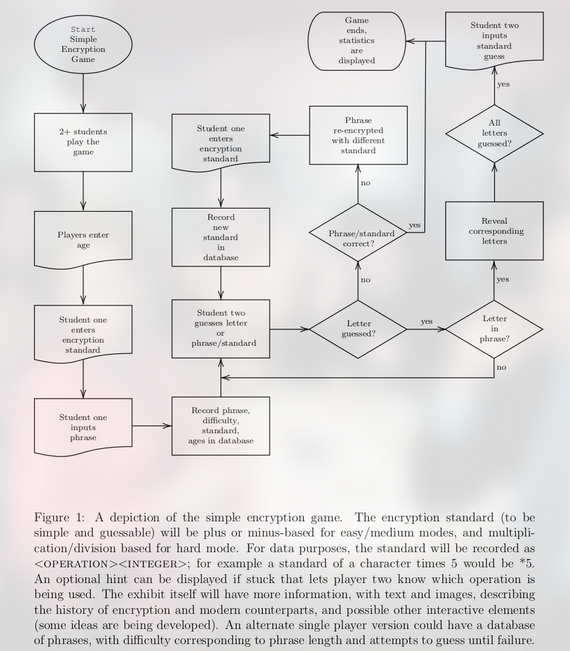
\includegraphics[width=.45\textwidth]{Figures/initLogic.png}
  \caption{Initial Game Logic}
\end{figure}

\subsubsection{Prototype}

\par When it came time to create the structure that would house our design, the original design was no longer compatible with what the ideal final outcome would be. As a result the design from appendix c was abandoned in favor of a more solid structure. As a result, a sturdier design was produced that housed a laptop with the code on one side with the LEDs, LCD screen, and bluetooth keyboard on the other. Wood was the ideal product for this design because it is sturdy enough to support the design but it can be cut easily. The biggest hurdle in this process was getting the LCD screen to fit perfectly in the wood, but the laser cutting requirement for this project was the perfect solution.  As visible in appendix G, the wooden structure has drilled holes with LED sockets for each bulb, as well as a laser cut rectangle for the LCD screen. The design is centered around two nearly identical hollow displays that each house one of the screens. The two halves are then placed together, hiding all of the hardware inside the hollow middle. To prevent participants from people exiting from the program during the exhibit, the keyboard was blocked off with wood and there was a slit to slide the keyboard under with the screen remaining exposed.  
\par While proving the concept, a main decision to be made was which Sparkfun elements to include in the design. The LCD screen was an obvious addition as it is necessary to display the encrypted message. A timer was necessary for this type of game so dedicating a sparkfun element to that was a given. Discussion led to the conclusion that LEDs would be the best way for someone to clearly see how much time they have left while not having to focus too much. As a result, a row of LEDs that turned off one by one in even increments depending on the allotted time was inserted. One additional element that was a possibility was a soundbox that played different sounds if the user won or lost. Unfortunately there was not enough time as there was difficulty finding the correct code to play the appropriate sound. However, this endeavor did lead to a visual element when someone won the game. Instead of a sound, the timer LEDs flashed when someone guessed correctly. You can see in the wire diagram that the final design included both a set of LEDs, a screen, and a knob for the screen brightness. In the attached gantt charts it is clear that the middle stages were all over the place as division of the code, research, and design responsibilities was unorganized. This contributed to one of the most prominent design challenges being organization because making sure each element was completed in time required a lot of discussion. 

\begin{figure}[H]
  \centering
  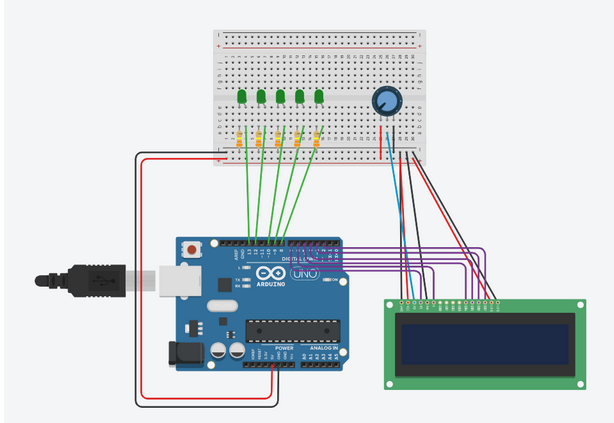
\includegraphics[width=.45\textwidth]{Figures/WireDiagram1.png}
  \caption{Wire Diagram}
\end{figure}

\subsubsection{Data Collection}

\par Following the in-class review of our preliminary design, it was clear the exhibit was lacking a definitive method of data collection. As a result, discussion around the basic methods like a QR code on the poster ensued, but something more concise and consistent was ideal as many people could miss a code. The solution was to embed collecting data within the code to make it mandatory before playing. The game itself tests the user’s ability to solve an encryption puzzle easily, so one of our data points being the time it takes to solve was a given. Along the same lines, a data point that could possibly correlate to the time it took to solve would allow for purposeful data analysis. The user’s age made the most sense to us as a lot of the educational research highlighted the ways exhibits should be less rushed with a lower age and we wanted to see if the same principle would apply for the interactive elements \cite{b16}. 

\subsubsection{Final}

\par Before conducting any sort of testing, the code had to be finalized to make it actually interactive. This step is where the sound option was officially abandoned and the method of stimulation became the LEDs. It is visible in the gantt charts that most of Henry’s time was allotted to the code in later steps as that was the biggest focus. Other than that, simply putting together the educational elements and cleaning up the wooden structure were the only responsibilities. In terms of education, prioritizing independence when playing a game was a must so there was a separate set of instructions included on top of the game structure so players could play on their own. For the poster, including information on necessary topics like ASCII was also a priority in order to familiarize any possible players with the method used to decrypt messages in the code.  

\subsubsection{Individual Contribution}

\par When it comes to the initial design of the exhibit my influence was fairly limited. My initial ideas focused too much on the educational and engaging aspects of the mission, leaving out essential factors like relation to spyware or interactivity. One of my ideas was designed to be an additional element to an exhibit rather than the main concept. My research indicated that keeping students engaged was an essential aspect of education \cite{b23}, so I came up with a fake invisible ink disaster. This idea, while interesting and engaging, did not apply to our chosen design. My other idea was based on a heel transmitter used by the KGB to inconspicuously record conversations. This idea was heavily focused on education surrounding the history of spyware \cite{b20} and lacked a viable interactive element. These ideas did not perform poorly in the decision matrix and were actually the two strongest designs behind the encryption game. The heel wiretap especially displayed some potential in problem areas like interactivity, but the encryption game was not only more attainable, but the concept as a whole was more complete. After the design had been chosen my role became a lot more prominent as we collaborated as a group to decide what elements had to be included. I suggested some elements we pursued, like the sounds correlating to success or failure, and others that ended up in the final product like the separate set of instructions. I was also heavily responsible for a lot of the research used to prove our concept, most notably the evaluation planning. This iteration was, personally, the most influential out of them all as it required me to have a complete understanding of our desired concept in order to create a plan surrounding data collection and its purpose in relation to the game. 

\newpage

\addcontentsline{toc}{section}{NEIL DUNGCA}

\vspace{10pt} \LARGE \textbf{NEIL DUNGCA} \normalsize

\subsection{Introduction}

\subsubsection{Problem Statement}

\par The primary goal of the project is to develop a museum exhibit that demonstrates and presents a topic within the theme of Espionage.  Objectives for the project involve a design that is educational, intuitive, interactive, accessible, and lightweight.  Because it is intended to teach users about a specific topic, it is of the utmost importance that the exhibit is able to educate users.  Additionally, users should not only be able to personally interact with the exhibit so that they can better learn from it, but user interaction should be intuitive so that minimal instruction is necessary for them to understand and use the exhibit.  In order to reach a wide range of audiences, the exhibit must also be accessible, catering to different ages, interests, and abilities.  Finally, a lightweight project would make for easier transport and setup.
\par In addition to the project objectives, the design must also adhere to specific constraints.  In terms of size, the exhibit must fit on a 36'' x 28'' table top while set up and inside of the provided container while in transit.  Designs should also be safe for set up and transport, include educational text about the concept, and be valued at less than \$1,000.  Finally, the design must incorporate arduino and matlab and include at least two elements from the SparkFun Inventor’s Kit.

\subsubsection{Stakeholders}

\par The main clients for the exhibit are Professor Brian O’Connell and the College of Engineering.  As a part of the stacked Cornerstone course, students must develop projects for the First Year Engineering Expo, which is run by Northeastern’s College of Engineering.  
\par The users for the exhibit are attendants of the expo who use and interact with the exhibit.  The design will benefit them by engaging and educating them.  By appealing to a wide audience, the design should not only inform, but excite users about the topic.  

\subsubsection{Scope}

\par The technical report outlines the team’s process from crafting a problem statement to developing a final product for the First Year Engineering Exhibition.  While the exhibit can be considered complete, it is not at a stage where it could be put forward for commercial use; materials are functional but not the most durable nor presentable.

\subsection{Background}

\subsubsection{Research}

\par The most pertinent research was information regarding existing, successful museum exhibits.  According to Brigid Laurie and John Powell, a major educational element of an exhibit is the “interpretive hierarchy.”  To teach a concept, an exhibit should start with a big idea.  Next, it should include some more specific key messages about that idea.  Finally, it should leave audiences with critical questions about the concept to spark further inquiry. \cite{b2} Another guide, the Exhibit Design and Development Workbook explains the elements of an exhibit that contribute most to information retention.  According to McMillan and Toxey, users remember 10\% of what they hear, 30\% of what they read, 50\% of what they see, and 90\% of what they do. \cite{b1} This finding led us to our determination that interactivity and intuitivity were key objectives of the project because users should be doing as much as possible to ensure they learn from the exhibit.   
\par Research for the project included information not only about museum exhibitions, but also about specific exhibit topics to inspire project ideas.  Some of the areas researched were stealth technology, invisible ink, and privacy monitors.  Similar to how stealth plane fuselages absorb and reflect incoming radar signals, an apparatus could be created that involves objects bouncing off of a user-made fuselage to test whether their design would be detected by a radar or not. \cite{b9} Invisible ink could be used to write a secret message and users could try to discover that message. \cite{b15} Finally, certain symbols could be displayed on a monitor that can only be seen when wearing polarized glasses. \cite{b3}

\subsubsection{Ethics}

\par Because the project is used by and presented to the public, it is important that it is safe and information is correct.  Sharp edges should be avoided and components of the exhibit should not be easily toppled over to reduce the risk of any users’ safety.  Additionally, the information being displayed to users should not provide false information, leaving users with skewed understanding of the topic.

\subsubsection{Universal Design}

\par The exhibit will be showcased to a diverse audience, so it is important that universal design is also taken into consideration.  Because users will be coming from different backgrounds and be of different ages and abilities, the exhibit must take these differences into account to cater to any user, allowing anyone to engage with the exhibit.

\subsection{Methodology}

\subsubsection{Understanding the Problem}

\par The group met to decide upon primary project goals, discuss the constraints of the design, and establish a problem statement.  Objectives included educational, intuitive, interactive, accessible, and lightweight.

\subsubsection{Ideation}

\par After conducting individual research, team members each came up with exhibit concepts.  Ranging from stealth simulations to wire-tap finders, hidden messages to encryption games, the concepts covered a wide variety of topics within the theme of Espionage. 

\subsubsection{Decision-Making}

\par To decide upon a concept to pursue, the group conducted a Kepner-Tregoe Decision Analysis (KTDA).  First, we ranked each project objective against each other to determine which goal was the most and least important; educational was ranked highest and lightweight lowest.  After applying weightings to each objective, we rated each exhibit concept for each objective, allowing us to calculate total scores for each design.  The multiplayer and single player encryption games earned the highest scores, leading the group to pursue that exhibit. 

\subsubsection{Implementation}

\par Initial models of the exhibit were created in SolidWorks before constructing a cardboard mock-up.  An initial prototype was then started.  Instead of having pieces cut by red vests in FYELIC, however, we attempted to cut scrap wood by hand, leading to uneven, splintering components.  Our next attempt, with the help of red vests, produced cleaner parts cut from bookstore wood that could be used for a prototype.  This version proved physically successful as it housed the laptop, LCD monitor, and arduino effectively.  To finalize the project, holes were drilled to house LED lights and the exhibit was painted for aesthetics.  
    \par The code for the exhibit went through many more phases.  For the first prototype, text was simply displayed to the LCD monitor reading ``enter guess.''  Later iterations were able to encrypt entered messages and display character input from the keyboard to the LCD display in live time.  The final code requests user name and age, encrypts an entered phrase, and displays that to decryptors while turning off LED lights to indicate time.  The users’ demographics are recorded to a text file along with the amount of time taken to guess their phrase.  

\subsubsection{Evaluation}

\par Before the First Year Engineering Exhibition, the exhibit was tested by the group and other members of the Cornerstone class.  Feedback was given primarily verbally.  Respondents suggested that the number of spaces the word has been shifted be displayed to decryptors and that the group include guidance for users in their poster board.  

\addcontentsline{toc}{section}{MALIGNITY OF GOBLINS}

\vspace{10pt} \LARGE \textbf{MALIGNITY OF GOBLINS} \normalsize

\subsection{Final Design}

\par The final exhibit includes two sides for encryption and decryption, and a poster board for information.  The encryption side includes a wooden base that holds a laptop, covering the trackpad.  The decryption side includes a wooden base, a bluetooth keyboard, a frame for an LCD 16x2 display, five LED lights, and a backing that stores the electronics.  Wooden pieces were cut to the following dimensions shown in figures \ref{fig:LC1} and \ref{fig:LC2} based on the size of the laptop:
\begin{figure}[H]
  \centering
  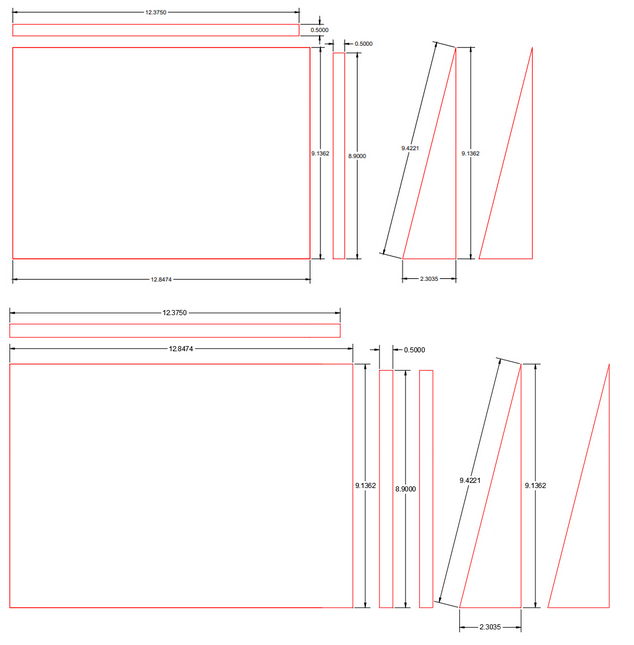
\includegraphics[width=.475\textwidth]{Figures/LaserCut1.png}
  \caption{First Two Laser-Cut Boards}
  \label{fig:LC1}
\end{figure}
\begin{figure}[H]
  \centering
  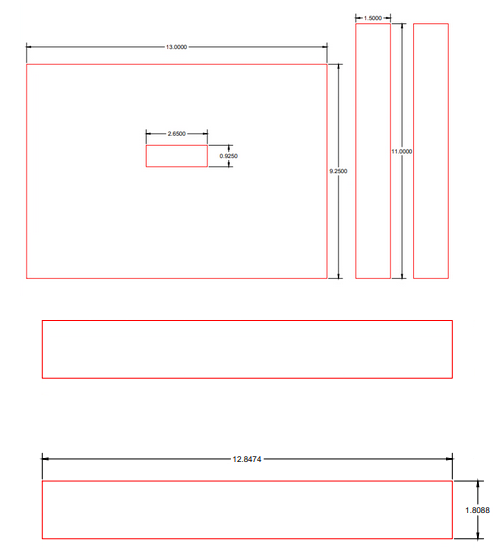
\includegraphics[width=.475\textwidth]{Figures/LaserCut2.png}
  \caption{Third Laser-Cut Board}
  \label{fig:LC2}
\end{figure}
\par The exhibit involves two users, one encryptor and one decryptor.  The encryptor begins by entering their name and age.  They are then prompted to enter a mystery phrase to be encrypted and select the amount of time in seconds for the decryptor to guess the phrase.  After clicking “encrypt,” the decryptor is presented with the encrypted phrase and the number of characters the letters are shifted.  The five green LEDs are lit and turn off at an interval one fifth of the selected guess time.  
Encryptors see a screen that displays the decryptor’s keystrokes live as they guess.  If the decryptor guesses the phrase correctly within the time, the lights flash indicating success.  Otherwise, the lights turn off and a message appears on the LCD screen saying that they did not guess the phrase in time. 

\subsection{Results}


\par Our design measures how long it took the user to solve the puzzle as well as their age. The users were able to set the time between 10 and 120 seconds but the solution times were all documented together. 
\par When it comes to analyzing the solution data, 13/32 of the participants were unable to solve the puzzle in time. Additionally, there is no clear correlation between age and ability to solve the encryption puzzle. 
\par For analytical reference, our code also documents the inputted phrase, what it was encrypted, and the number of digits the ASCII value reversed by. This allows for the comparison of phrases of similar length, of similar digit rotation, or both. 

\newpage

\addcontentsline{toc}{section}{HENRY SHIELDS}

\vspace{10pt} \LARGE \textbf{HENRY SHIELDS} \normalsize

\subsection{Discussion/Analysis}

\par The device overall operated successfully. During the performance of the design, there were two shortcomings, one in the form of difficulty, which was adjusted by displaying the exact ASCII value the phrase had been rotated by, and a bug wherein the user presses encrypt multiple times in a row, which entirely crashes the program. However, the former was fixed on the spot and the latter is a matter of adding essentially a cooldown timer. While annoying, these matters proved rare and insignificant in the evaluation of the device. The encryption machine perfectly fit the size and weight constraints as it objectively fit in the provided box and did not exceed the given weight. Furthermore, the resilience of the device was apparent seeing as it is still in mint condition and working properly, though this was not necessarily tested to completion. The visual accessibility was successful as the laptop lid was foldable/adjustable, and the LCD Display was at a level and contrast where it was visible from every angle the users tested during the exhibit. As for electronics, the device most certainly used the required programs and number of peripherals as outlined. Measuring a value such as teamwork and education proved somewhat harder, however, in interpreting the users’ interactions, there was very little teamwork as players approached in groups of two and simply played “against” each other one-on-one. I would say that the device somewhat failed to inspire teamwork in this regard, although it certainly had the capabilities to do so. As for education, I had multiple talks explaining ASCII values and how the code works, which, combined with our poster on the history and modernity of encryption, I would evaluate the design as successful in efficiently educating the users. In displaying the exact ASCII value, the device also became more accessible to younger kids, who similarly to older students, can track the given ASCII chart to decipher the phrase. This combined with the simple but useful instructions and variable layers of the poster board, the device was very successful in being interactive and enjoyable for all ages. 

\subsection{Conclusion}

\par The final design had the user enter their age and name which were recorded to a text file on the laptop. They then inputted a secret phrase and selected a time for the opponent to solve against and click encrypt. From here, a row of LED lights lit up on the opposite side where the person decrypting sat, these lights ticked down according to the timer previously specified. The user is then given the encrypted code and the number that each ASCII value was rotated by. Using the printed chart and the given encryption, the user actively types in the guess, with it being displayed on the LCD monitor before them. If they successfully type in the guess then the LEDs flash on and off consecutively and a congratulation is displayed with the time it took to solve, which is written to the text file previously mentioned. If the lights all turn off before the word is guessed, then the user is displayed a losing message and the time is recorded in the text file as 0. All in all, the device functioned successfully and effectively in its testing environment. The users were entertained and learned something about codebreaking and ASCII values in code. It successfully educated and entertained the target audience of students of all ages. Fitting nearly every constraint perfectly and staying under the budget of 100 dollars, I would call this device a success, though like most designs it has room for improvement. Such examples would be incorporating audio, changing the material to metal, and refining the code.

\subsection{Recommendations}

\par In evaluating a redesign of this project, there are a number of factors that could stand to be improved for future or even professional use. The first of which is the implementation of a buzzer or the sound() function by MATLAB. Simply due to time constraints and priorities, the goal of an audio based indicator of correct or incorrect in the encryption device failed. The buzzer was initially causing issues when interacting with the LCD Add-on Library, however, even with professional consulting, the issue could not be resolved and the function sound() was not used to its full potential. This would then be the first change that would add to the accessibility of the design. Secondly, there is a somewhat awkward gap between entering the hidden phrase and the displaying of it on the LCD Monitor on the other side of the device. This is due to a segment of code that is running in a loop during the time in which the user attempts to enter their guess. It does not hinder the functionality of the device, however, it feels clunky. This should be debugged and changed to a state where the program can multitask entering the input. The final design suggestion for this project in future development would be replacing the materials with possibly metal or better wood simply for aesthetics. The finished design from the malignity of goblins was sanded and smooth however hot-glue was still visible in places, the dowels were not flush with the top of the device, and the LCD Monitor slot which we had to cut out via hand-saw, were chipping. By replacing the wood with bent and soldered metal, a much cleaner product could be created, not to mention the increased durability. Perhaps even a hinge could be implemented to open up the electronics compartment.

\subsection{Lessons Learned}

\subsubsection{Individual Contribution}

\par Through this project, I learned an enormous amount about the engineering design process as well as physical skill sets utilizing Arduino and MATLAB. In creating this project, I did the vast majority of electronics and coding, which was time-consuming but fantastically educational. I learned to approach problems from many different directions as there were constant roadblocks to the process of creating a final product. For instance, in using the LCD Monitor provided by the Spark Fun Engineering kit with the MATLAB App creator, I had to manually install a library. However, when that library was not suiting my needs accordingly, I adjusted the methods within it, which was outside my comfort zone, but very interesting. Another such roadblock was the Piezo buzzer, which for hours was simply interfering with other pins and refusing to work, which led to the approach of using the sound() command in MATLAB. Digressing from the software part of this project, I also learned how to wire an LCD Monitor in a breadboard and use premade LED resistors that served as the basis for the LED timer in the final product.   

\subsubsection{Group Evaluation}

\par However, besides building and coding the final design, the engineering design process was approached and evaluated as a group. I believe that we allocated our time, money, and other resources accurately and efficiently. The work was divided by who had the most experience and interest in each department of engineering. Therefore, as a computer engineering and computer science major, I took electronics and software, whereas other members took the physical product (woodworking, mechanics, etc.). Every memo was completed on time, though my criticism is that on numerous occasions, while not wasting resources, the group left work for the last day which led to crunch work. This is inefficient in evaluating the quality of the final product and if a new project was approached, I believe our allocation of time, not work, could be beneficial to the stress and quality of our product. However, there was no money wasted, tasks redone because of mistakes, or clear violations of requirements and so all in all, I would argue that The Malignity of Goblins was generally efficient and successful in our allocation and utilization of resources. In addition, as a participating member of an engineering group, this was a fantastic first experience as the team dynamic was welcoming, friendly, and humorous. There was never any held-back information for fear of shame or embarrassment, we openly shared and that led to a much better design than any one of us could have achieved alone. 

\subsubsection{Takeaways}

\par Throughout this effort, my understanding of the engineering design process expanded greatly. Firstly, with background research and understanding of the mission, a problem definition with constraints, stakeholders, and goals Through group brainstorming and research exchanging we created numerous solutions to the given problem and decided upon the best option via a rank order and KTDA chart. Which was then implemented according to our plan through MATLAB and Arduino. This only leaves technical and engineering communication, part of which is learned and achieved via this very technical report. However, these skills were also honed via the Town Hall presentations in which our engineering design process was written out to be understood clearly, and in the status memos, in which our process was documented officially. 

\newpage

\addcontentsline{toc}{section}{MICHAEL BRODSKIY}

\vspace{10pt} \LARGE \textbf{MICHAEL BRODSKIY} \normalsize

\subsection{Discussion/Analysis}

\par All in all, despite improvisations and problems encountered along the way, the design worked quite well. Although the design was quite different from what I envisioned originally, I think it turned out even better. As indicated by the near-constant queue to partake in the encryption game, people were clearly engaged and interested to learn about encryption. The fact that our project involved someone on both sides of the table made it quite unique and differentiated from others; additionally, the information regarding encryption, both contemporary and historical, made people more likely to see the project and have their interest piqued.
\par The biggest concern with the project is probably that it is a bit difficult to win. As shown by figure \ref{fig:4}, 18 out of the 32 total games resulted in a loss, as indicated by a time of 0. This means that the winning percentage is $\nicefrac{1400}{32}$, or $43.75\%$. The best change would probably be to display the exact number the characters were shifted by, instead of a range of characters. This way, decrypted the phrase with the ASCII-value table provided becomes much more feasible in the given time frame.

\subsection{Conclusion}

\par Overall, it is evident that the project functioned quite well due to the high level of engagement. As such, it seems that the project was quite successful in fulfilling its requirements
\par In regards to the actual constraints, the exhibit meets all of them. The project is safe, both during use and transportation, follows the theme of espionage technology, easily broken down, costs less than \$100, can handle regular interaction, is engaging and educational, and collects user data to indicate success.
\par In this manner, the project not only fulfilled the requirements but also went above and beyond, as it was also highly accessible, and fairly lightweight.

\subsection{Recommendations}

\par Given more time and resources, I would definitely try to model it more after my initial design, but with the code of the current design. By modifying the device to have two touch-screen monitors with the ability to run a basic graphical user interface-based application, the device will be significantly more portable, in addition to no longer relying on a laptop. In this manner, the product will be much easier to use, as well as a bit more accessible.
\par Additionally, I would also add some kind of noise, especially when the phrase is guessing. Albeit the flashing lights are a bit entertaining, having the device make sounds would make it more appealing, especially to kids, thus increasing the amount of engagement.
\par The biggest problem with designing the product is that we did not have a full grasp on our resources and how to delegate them. Accordingly, as was previously mentioned with the limited amount of pins, which led to the use of a single monitor, instead of dual monitor game system, would have been mitigated had we better anticipated this. In this manner, I will better understand resource management for similar future products.

\subsection{Lessons Learned}

\subsubsection{Contribution}

\par Although I did contribute to building the project itself, assisting with the wiring, and memorandum production, my biggest contribution was easily this document. With more than 20 hours of effort, I modified the IEEE \LaTeX template to better accommodate the requirements laid out in the example report. In doing so, I created a well-laid-out, professionally typeset document, in accordance to IEEE standards.
\par In terms of the specifics, I first and foremost had to modify the title page to include images and all authors. This was fairly easy; however, modifying the existing structure to change how section and subsection headers were displayed, as well as how the table of contents was printed took a while. Every table, originally produced in an online editor so that the team could edit simultaneously, was also reformatted into tabular format within \LaTeX. Additionally, the attached Gantt Chart (see \ref{GC}), was entirely generated in tikz. The underlying code to all of these, as well as all class assignments, will published after the end date of December 9, 2022.
\par This has been quite beneficial, as I have learned about a lot of new functionality in \LaTeX, as well as many existing packages.

\subsubsection{Resources}

\par Although it was a bit close, as shown in \ref{table:4}, the group did meet the financial spending limit. The team was organized so that one person purchased all of the products, in order to make it easier to later determine how much everyone owed, so I did not personally acquire any of the products. If I had to estimate overall, I have probably dedicated at least 100 hours total. This project has given me a lot of insight into how to plan resource management. More specifically, I never thought it reasonable to start allocating and planning for resource usage before even deciding on a design, but given the nature of electronic components, one project can easily be turned into another, meaning it is still possible to plan which parts will be needed.

\subsubsection{Reflections on Learning}

\par Throughout this project, I have learned the most about MATLAB integration with Arduino. Despite this being possible, I have learned a lot about how there isn't always a 1:1 command that matches something within Arduino. This caused the most hardship when we were trying to implement the LCD, which, little did we know, required a separate MATLAB Add-on. As such, I learned a lot about how to the behavior of MATLAB when used with an Arduino. 
\par Additionally, I simply learned a lot about working in a team. A lot of this was learning how to lead and organize my team, so that we can be as efficient and as responsive to contact as possible. Both of these skills will be very helpful throughout my career.


\subsubsection{Reflections on Working in a Team}

\par To be honest, I found it quite easy to work on this specific team. Because all of the members were quite open to constructive criticism and improvise, we were able to be quite successful. I would not say the project changed my team working skills, but rather improved my existing ones. Because of the significant portion of the class dedicated to work produced as a team, we had a group incentive to work as best and efficiently as possible.
\par The most difficult part of this, for me, was not being leader. Because I generally want to organize and plan ahead, I usually want to take the lead on projects. Thus, it was difficult, albeit not impossible, for me to step down for a while during other members' turns to be project managers. I was able to adapt though, and allowed other members to lead.
\par As a team, overcoming adversity was not too much of a problem. Our technique was simple: everyone played to their strengths. In doing so, we were able to efficiently delegate tasks, thus allowing for quicker, but still quality, completion of assignments. Our biggest asset was definitely our resolve and willingness to work, especially as a team. To be honest, if I had to start from scratch, there is not too much I would change. The only thing I can think of is try to caution the team to learn of each others' abilities as soon as possible. As stated in my Recommendations, given more time and resources, I would want to make the project as I initially envisioned — a more portable, two-display version.

\newpage

\addcontentsline{toc}{section}{MICHAEL LEVY}

\vspace{10pt} \LARGE \textbf{MICHAEL LEVY} \normalsize

\subsection{Discussion/Analysis}

\par The results provide evidence that the design was very effective in being interactive while allowing users to make it as challenging as they’d like. The results vary greatly and show that some users were able to solve their puzzle within seconds, and others could not solve it at all. A challenge while creating this design was ensuring that both players were engaged throughout the game’s duration, but seeing how much the results vary clarifies that the encryptors were very engaged when creating phrases and while setting the time limit. The goal of consistent interest is definitely fulfilled after reviewing the data and taking note of how creative those using the device got. 
\par The design was very successful in fitting most of the constraints as well. There was no issue fitting it inside the provided tub and it was easy to set it up in less than a minute. The design also clearly utilized multiple sparkfun elements, as both the LCD screen and LED lights are reliant on the arduino. However, the price restraint is where difficulties arose. Due to materials already possessed, staying under the budget was possible, but a lot of the necessary technology is more than the budget allotted for. When adding all of the materials obtained from FYELIC for free, the original amount spent of $85.76 would exceed the budget of $100. This is not including the required Sparkfun materials or the laptop required to run the code. 

\subsection{Conclusion}

\par The exhibit was very efficient in terms of fulfilling the goals outlined in the introduction. Most notably, the goal of accessibility was met as there was nobody at the expo that wanted to interact with the encryption game but could not. Similarly, the expectation of education was of little concern as people had no issue grasping the game’s concept and trying to decrypt the message. The data, however, may suggest that the game may have been difficult at times considering how many users were unable to solve the puzzle. Additionally, upholding the reputation of our academic stakeholders was achievable because the design worked bug-free and the group was able to answer all questions that were asked of us throughout the exhibit. 
\par In terms of the performance of the device, overall it was extremely successful. It was easy to allow many users to play the game consecutively and each time the game ran without issue. There was a slight issue when users tried to tap the “encrypt” button too many times, but the arduino simply had to reconnect and the user would then press it one more time. Some of the previously troublesome elements of the device like the LEDs ran without fail and successfully counted down for every user, as well as lit up again for those that solved the puzzle. 


\subsection{Recommendations}

\par The biggest recommendation for a project like this is to decide how the device would ideally function before starting any of the building elements. While the initial design may not end up being feasible, there will still be clear functions of the design that can be achieved through iteration as the design goals were already clarified. When designing this game, some elements like the LEDs seem like a necessity, but were not something that was originally planned. Rather than just stating that the designs should have something like a timer when planning, come up with a few ideas of what that timer could be. That preparation will allow you to think of how to implement elements while building, rather than after the fact. 
\par When it comes to this project, some areas definitely fall short in terms of accessibility. Due to time restraints,  it was necessary to reorder the design goals, and accessibility consistently fell further down the list. However, if there was more time when creating this design there ideally would have been an audio element to let users know when they solved (or failed to solve) the puzzle in case they were visually impared. Similarly, there would have been a braille version of the ASCII table in order to increase accessibility as that was originally our most prevalent goal. 
\par In terms of commercializing this design, the biggest recommendation is to create a more secure 
circuit. While there were few issues with this one, there are many wires connected to the arduino, all of which are necessary for the device to function. Finding a way to hide the circuit while also keeping it stable would be a requirement for mass production. Similarly, connecting a keyboard to the decryption side and the LCD screen would eliminate the need for a bluetooth keyboard and would minimize concerns surrounding external devices like battery life and connectivity issues.

\subsection{Lessons Learned}

\subsubsection{Contributions}

\par A large part of my involvement in milestones 5-7 was based in organization and completing extraneous tasks. When it comes to milestone 5, a lot of my effort was allocated towards the momo’s organization as I was the most familiar with many of the traditional memo elements. Updating the problem statement to reflect a shift in focus from accessibility to audience engagement was the first task. Another notable section was the compilation of photos throughout the entire project to formulate a photo log. I had been responsible for delegating which tasks would be completed in which milestone so it was also my responsibility to divide the photos between milestones. 
\par When looking at milestone 6, I was responsible for spearheading the memo and evenly splitting the exhibit analysis between the group. As I had conducted most of the research on education methods, I wrote about the primary educational elements of the exhibit. Mentioning how the extraneous elements, like instructions board and ASCII table, provided users with all the information needed to play clarified how the goals of education and independence were accomplished. In terms of the exhibit itself, I was responsible for putting together the poster for our exhibit as well as the additional elements like the ASCII table and set of instructions. I was also focused on familiarizing myself with the memo requirements and distributing the elements between group members. 
\par The milestone 7 contributions were different from those in the previous milestones because they were more focused on collected data rather than education and design. Aside from the individual tasks, I handled the results aspect in section 1.14 of this report and finalized appendix D, the product testing results

\subsubsection{Resources}

\par Due to our group already possessing most of the expensive elements, we were able to stay within our budget for this project. In total we spent \$51.47 on laser-cutting wood, our poster, a bluetooth keyboard, and painting supplies. However, if we did not have the more expensive elements like the sparkfun kit and the computer our cost would have been upwards of \$1,200. While planning our budget for this project I realized the importance of defining the extraneous parts of your design in the initial stages so you know what to expect when you are actually building them. By the time we had settled on elements like the LEDs for our timer a lot of our budget had been distributed and we had to adjust it for everything to fit. If we had a better idea of the things we had to purchase in the earlier stages our budget could have been far more defined earlier on. Instead, it was like we had a completely different bill of materials for every milestone.

\subsubsection{Reflections on Learning}

\par The biggest takeaway I have from this project is experience having such a broad assignment and being tasked with keeping myself on track while meeting each deadline. Up until this point my hand has been held in projects like this so I had to teach myself how to plan tasks ahead weeks in advance and how to set a schedule my group and I could realistically stick to. I certainly gained a lot of valuable experience in terms of both organization and leadership that will be beneficial in future endeavors. 

\subsubsection{Teamwork}

\par Throughout this project I certainly had to adapt my work style to help my group function efficiently. A lot of my group members work at a much faster pace than I do and therefore don’t start a lot of their tasks until after I have. As a result, a lot of the memo was my responsibility as it allowed me to start working as early as I’d like while not leaving my group out of decisions. My leadership style is heavily focused on equal opportunity and I hate working in a way that feels like one person is taking charge over everyone else. However, this mindset sometimes backfired as I had to stay up later than I’d like finalizing a memo because a group member had not yet worked on it. This process taught me that I can be assertive without being overbearing.

\newpage

\addcontentsline{toc}{section}{NEIL DUNGCA}

\vspace{10pt} \LARGE \textbf{NEIL DUNGCA} \normalsize

\subsection{Discussion/Analysis}

\par The most notable take away from the data collected is that only 43.75\% of users - many of whom were members of the group - were able to guess the encrypted phrase.  This seems to suggest that the exhibit was too difficult to understand, meaning that it was not fully intuitive and interactive for users, potentially leading to poor education of information relating to encryption.  
\par Additionally, user ages ranged from 17 to 21 years old.  With the given success rate in this age range, it can be reasonably assumed that the exhibit would also be too difficult for younger users in a children’s museum. 

\subsection{Conclusion}

\par Overall, the project appears to have been mostly successful.  Despite a low guess rate for users, the exhibit still functioned properly within the size, technology, and price constraints.  Additionally, the poster board presented relevant information to the topic of Encryption.  The main fallback is the difficulty of the game which contributes to potentially unproductive (users were not able to learn from the exhibit) interaction with the exhibit.

\subsection{Recommendations}


\par The physical design of the exhibit could be greatly improved.  With an increased budget, a larger screen could be used to display more information to decryptors; the encrypted phrase, time remaining, number of characters shifted, and instructions could all be displayed at once.  Additionally, the base could be constructed of stronger materials.  The wood currently being used is simply glued together and has splintered, leading to possible compromise of the structure’s integrity.  If the components were more strongly put together - bolted, screwed, or even welded - or stronger materials - thicker wood or metal - were used, the exhibit could be much more durable and presentable.  
\par Improvements to the software of the exhibit include updating the encryption interface to be more aesthetically pleasing and providing better instructions to decryptors.  With further instruction, the guess rate should increase, leading to more user interaction that leads them to an understanding of how encryption works.

\subsection{Lessons Learned}

\subsubsection{Contributions}

\par Since the 90\% prototype of the exhibit, my most significant contributions have been to the physical build and aesthetics of the project, resource management, the wire diagram, and updates to the problem statement.  I was largely responsible for having wood cut for the components and assembling the physical structure.  Additionally, I painted and took photos of the exhibit.  For the proof of concept, I created a wire diagram including the LCD monitor and LED lights in Tinkercad.  Finally, I worked with the team to determine updates for the problem statement.

\subsubsection{Resources}

\par The value of the exhibit’s components totaled to \$130.31, as shown in \ref{table:4}. Of the materials purchased, I spent \$85.76 for the wood, paint, brush, and wireless keyboard.  While I did not spend the most time on the project because of the sheer number of hours spent coding, the effort dedicated to constructing the exhibit should be comparable.  
\par My biggest takeaway from the resource management throughout the project is that there are many things to maintain track of during a project.  From photos to hours to prices, it is important to be on top of every aspect of the process.

\subsubsection{Reflections on Learning}

\par Over the course of the project, I have become much more proficient at communicating ideas effectively through status memos.  Additionally, I learned how to more effectively construct models from wood, taking advantage of the resources at FYELIC.  While woodwork may not contribute to a career in Chemical Engineering, knowing how to access and use the resources of a workshop can be hugely beneficial, especially if I am unable to physically create certain prototypes myself.  

\subsubsection{Reflections on Working in a Team}

\par While still collaborating on aspects pertinent to the whole group, the team largely functioned by dividing tasks and working individually.  This has largely been how I worked with teams in the past and it appears to have been successful for the project.  The role of Project Manager, however, has definitely increased my awareness of the jobs of every team member; I’ve learned the importance of knowing how each individual task plays a role in the whole project.  If I could start this project again, I would make myself more aware of my group members’ tasks so I could fully understand the progress of the project.
 \par   While rare, any conflicts within the group were usually over simple misunderstandings of Milestone instructions.  These were resolved by consulting the instructions or asking members of other groups.  
 \par   My most significant contribution to the team was the building and logging of the exhibit.  From purchasing materials to dimensioning components, having pieces cut to assembling them, the physical exhibit was largely my responsibility.  With more time, I would have hoped to be more involved in the educational aspects of the exhibit and logic for the code of the game.

\onecolumn

\begin{thebibliography}{00}
    \normalsize
  \bibitem{b1} A. Toxey and P. McMillan, “Exhibit Design and Development Workbook,” \textit{Toxey/McMillan Design Associates}, 2009. 
  \bibitem{b2} B. Laurie and J. Powell, “A Guide to Exhibit Development,” \textit{Smithsonian Exhibits}, Apr-2018. 
  \bibitem{b3} C. Sorrel, “For your eyes only: Polarizing privacy monitor mod,” \textit{Wired}, 28-Nov-2011. [Online]. Available: \href{https://www.wired.com/2011/11/for-your-eyes-only-polarizing-privacy-monitor-mod/}{https://www.wired.com/2011/11/for-your-eyes-only-polarizing-privacy-monitor-mod/}. [Accessed: 18-Oct-2022].
  \bibitem{b4} “Cryptography.” Wikipedia. \href{https://en.wikipedia.org/wiki/Cryptography}{https://en.wikipedia.org/wiki/Cryptography}  (accessed: Oct. 18, 2022).
  \bibitem{b5} “Edge exhibit designs for girls' engagement,” \textit{Exploratorium}, 12-Nov-2021. [Online]. Available: \href{https://www.exploratorium.edu/education/research-evaluation/edge}{https://www.exploratorium.edu/education/research-evaluation/edge}. [Accessed: 18-Oct-2022].
  \bibitem{b6} E. Fox , “Accessible exhibitions for all - historyof.place,” \textit{History of Place Project}. [Online]. Available: \href{http://historyof.place/wp-content/uploads/2018/11/HOP\_TK\_Design\_Exhibs\_Final\_PRINT.pdf}{http://historyof.place/wp-content/uploads/2018/11/HOP\_TK\_Design\_Exhibs\_Final\_PRINT.pdf}. [Accessed: 18-Oct-2022].
  \bibitem{b7} “Exhibits — International Spy Museum.” The International Spy Museum.  \href{https://www.spymuseum.org/exhibition-experiences/}{https://www.spymuseum.org/exhibition-experiences/}  (accessed: Oct. 18, 2022).
  \bibitem{b8} G. Montsho, “Making museums accessible to those with disabilities,” \textit{MuseumNext}, 25-Jun-2022. [Online]. Available: \href{https://www.museumnext.com/article/making-museums-accessible-to-those-with-disabilities/}{https://www.museumnext.com/article/making-museums-accessible-to-those-with-disabilities/}. [Accessed: 18-Oct-2022].
  \bibitem{b9} G. Wollenhaupt, “How F/A-22 raptors work,” \textit{HowStuffWorks Science}, 02-Aug-2020. [Online]. Available: \href{https://science.howstuffworks.com/f-22-raptor.htm}{https://science.howstuffworks.com/f-22-raptor.htm}. [Accessed: 18-Oct-2022]. 
\bibitem{b10} “Interactive Exhibits — Creative Machines.” Creative Machines.  \href{https://www.creativemachines.com/interactive-exhibits}{https://www.creativemachines.com/interactive-exhibits}  (accessed: Oct. 18, 2022).
\bibitem{b11} J. Richardson, “How to design an exhibition: These 5 tips should be your Mantra,” \textit{MuseumNext}, 11-Aug-2022. [Online]. Available: \href{https://www.museumnext.com/article/designing-exhibition-5-tips-mantra/}{https://www.museumnext.com/article/designing-exhibition-5-tips-mantra/}. [Accessed: 18-Oct-2022].
\bibitem{b12} “Mapping gender equality in STEM from school to work,” \textit{UNICEF Office of Global Insight \& Policy}, 20-Nov-2020. [Online]. Available: \href{https://www.unicef.org/globalinsight/stories/mapping-gender-equality-stem-school-work}{https://www.unicef.org/globalinsight/stories/mapping-gender-equality-stem-school-work}. [Accessed: 18-Oct-2022].
\bibitem{b13} M. F. Mortensen, “Analysis of the Educational Potential of a Science Museum Learning Environment: Visitors’ experience with and understanding of an immersion exhibit.”
\bibitem{b14} International Journal of Science Education, vol. 33, no. 4, pp. 517-545, 2010, doi: 10.1080/09500691003754589.
\bibitem{b15} Michigan State University, “Cold War Invisible Ink Secrets Unlocked,”  \textit{ScienceDaily}, 08-Nov-2006.
\bibitem{b16} M. S. U. E. Kylie Rymanowicz, “Monkey see, monkey do: Model behavior in early childhood,” \textit{MSU Extension}, 17-Mar-2021. [Online]. Available: \href{https://www.canr.msu.edu/news/monkey\_see\_monkey\_do\_model\_behavior\_in\_early\_childhood}{https://www.canr.msu.edu/news/monkey\_see\_monkey\_do\_model\_behavior\_in\_early\_childhood}. [Accessed: 18-Oct-2022].
\bibitem{b17} P. R. N. Atlas, “KGB spy shoe with Heel Transmitter,” \textit{New Atlas}, 10-Nov-2016. [Online]. Available: \href{https://newatlas.com/kgb-spy-shoe-with-heel-transmitter/1576/}{https://newatlas.com/kgb-spy-shoe-with-heel-transmitter/1576/}. [Accessed: 18-Oct-2022].
\bibitem{b18} R. J. Batvinis, “Spy Satellites and Other Intelligence Technologies that Changed History”. By Thomas Graham Jr. and Keith A. Hansen. (Seattle, Wash.: University of Washington, 2007. Pp.ix, 162. \$14.95.).” The Historian, vol. 71, no. 1, pp. 111-112, 2009, doi: 10.1111/j.1540-6563.2008.00233 14.x.
\bibitem{b19} S. Fourtané “Spy Technologies used from WW1 through the Cold War in exhibition at the world's First Spy Museum in Finland,” \textit{Spy Technologies Used from WW1 through the Cold War in Exhibition at the World's First Spy Museum in Finland}, 22-Dec-2018. [Online]. Available: \href{https://interestingengineering.com/innovation/20th-centurys-spy-technologies-at-the-worlds-first-spy-museum}{https://interestingengineering.com/innovation/20th-centurys-spy-technologies-at-the-worlds-first-spy-museum}. [Accessed: 18-Oct-2022].
\bibitem{b20} “Shoe with Heel Transmitter,” \textit{International Spy Museum}. [Online]. Available: \href{https://www.spymuseum.org/exhibition-experiences/about-the-collection/collection-highlights/shoe-with-heel-transmitter/}{https://www.spymuseum.org/exhibition-experiences/about-the-collection/collection-highlights/shoe-with-heel-transmitter/}. [Accessed: 18-Oct-2022].
\bibitem{b21} \textit{Spyscape}, “Spy Cameras, Tech, Tools & Tales of the international spy,” SPYSCAPE. [Online]. Available: \href{https://spyscape.com/article/tech-tools-and-tales-of-the-international-spy}{https://spyscape.com/article/tech-tools-and-tales-of-the-international-spy}. [Accessed: 18-Oct-2022].
\bibitem{b22} “Top secret - imagine exhibitions.” [Online]. Available: \href{https://www.imagineexhibitions.com/exhibitions/top-secret}{https://www.imagineexhibitions.com/exhibitions/top-secret}. [Accessed: 19-Oct-2022].
\bibitem{b23} “Universal Design for Museum Learning Experiences,” Museum of Science, Boston.  [Online]. Available: \href{https://www.mos.org/UniversalDesign}{https://www.mos.org/UniversalDesign}. [Accessed: 18-Oct-2022].
\bibitem{b24} “What is edutainment? tips for mixing education and entertainment in the classroom,” \textit{What Is Edutainment? Mixing Education and Entertainment | American University}. [Online]. Available: \href{https://soeonline.american.edu/blog/what-is-edutainment}{https://soeonline.american.edu/blog/what-is-edutainment}. [Accessed: 18-Oct-2022]. 
\bibitem{b25} X. C. Zhang, H. Lee, C. Rodriguez, J. Rudner, T. M. Chan, and D. Papanagnou, “Trapped as a group, escape as a team: Applying gamification to incorporate team-building skills through an 'escape room' experience,” \textit{Cureus}, 02-Mar-2018. [Online]
\end{thebibliography}

\twocolumn

\addcontentsline{toc}{section}{AUTHOR BIOGRAPHIES}

  \LARGE \textbf{Author Biographies}  

  \vspace{15pt} \normalsize


  \begin{wrapfigure}{l}{.225\textwidth}
    \includegraphics[width=.175\textwidth]{<Headshot>.png}
  \end{wrapfigure}
  \par \textbf{Henry O. Shields} was born in Rochester, NY in 2004. He is an undergraduate student pursuing a B.S.\ in computer engineering and computer science with minors in mathematics and business administration from Northeastern University, Boston, MA, expected in 2026.
\par His interests concern the development of computer technologies such as that of AI, nanotechnology, and robotics.
\par Mr. Shields is a member of IEEE, Roxbury Robotics, and NUHOC.

  \begin{wrapfigure}{l}{.225\textwidth}
    \includegraphics[width=.175\textwidth]{Figures/headshot.png}
  \end{wrapfigure}
  \par\textbf{Michael D. Brodskiy} was born in Walnut Creek, California in 2004. He will receive a B.Sc.\ in Physics \& Electrical Engineering from Northeastern University, Boston, MA, in 2026.  
\par In 2022, he was a Research Assistant at the Northeastern University Institute for the Wireless Internet of Things, working on the use and detection of 5G+ signals and generation of wireless signal strength heat maps. He is a great supporter of the Free Software Foundation, and has published articles in his school magazine relating to digital freedom. He hopes to engage in nuclear physics in the future, and to attain a Ph.D.\ in this very field.
\par Mr. Brodskiy is currently a member of Roxbury Robotics, volunteering at the Paige Academy Jr.\ site, as well as a Northeastern Honors Scholar, and part of the UPLIFT program. Mr. Brodskiy hopes to eventually become an IEEE member.  

  \begin{wrapfigure}{l}{.225\textwidth}
    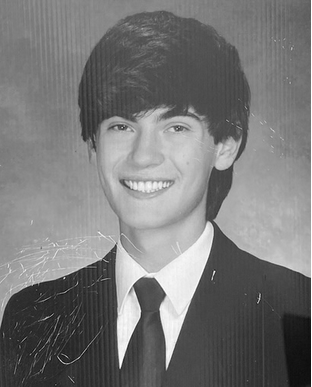
\includegraphics[width=.175\textwidth]{Figures/LevyImage.png}
  \end{wrapfigure}
  \par \textbf{Michael Levy} was born in Morristown, New Jersey, in 2003. He graduated Randolph High School in 2022 and is currently attending Northeastern University. 
\par    From 2020 to 2022 he was a tutor and had to research some basic engineering concepts to help one of his students. What he came across interested him and, as he was already looking to declare a major, decided on engineering. 
   \par Mr. Levy is currently a member of the Roxbury Robotics club at Northeastern and recently finished a cycle working with students at Yawkey Boys and Girls club. 

  \begin{wrapfigure}{l}{.225\textwidth}
    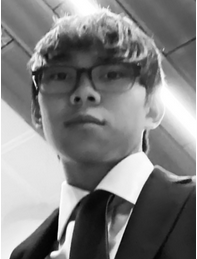
\includegraphics[width=.175\textwidth]{Figures/DungcaImage.png}
  \end{wrapfigure}
  \par \textbf{Neil Dungca} was born in Providence, Rhode Island, in 2004.  He graduated from Bishop Hendricken High School in 2022 and is a candidate for the Bachelor of Science in chemical engineering at Northeastern University, as a member of the class of 2026.  
\par In fall of 2022, he began working as a research assistant as a part of the Professor Steve Lustig lab at Northeastern.  He has dissected kevlar shoot packs from DuPont to be prepared for study of the mechanical properties of individual, broken fibers.  
\par Mr. Dungca is a member of the Northeastern University Honors Program, UPLIFT Program, and an intramural volleyball team.

\onecolumn

\addcontentsline{toc}{section}{APPENDICES}

  \LARGE \textbf{APPENDICES}  

  \newpage

\addcontentsline{toc}{subsection}{Appendix A — Team Contract}

\Large \hspace{.5in} \textbf{APPENDIX A — TEAM CONTRACT}
\normalsize (See next six pages) \Large

\includepdf[pages=-,scale=.95]{Figures/Contract.pdf}

\addcontentsline{toc}{subsection}{Appendix B — Decision Analysis} 

   \hspace{.5in} \textbf{APPENDIX B — DESCISION ANALYSIS}  

   \begin{table}[H]
     \centering
     \begin{tabular}{| l | r | r | r | r | r | r |}
       \hline
       \textcolor{darkgray}{Rank Order} & \cellcolor{black} & \cellcolor{black} & \cellcolor{black} & \cellcolor{black} & \cellcolor{black} & \cellcolor{black} \\
       \hline
       \textbf{Objectives} & Educational & Interactive & Accessible & Intuitive & Lightweight & Sum\\
       \hline
       Educational & \cellcolor{gray} & 1 & 1 & 1 & 1 & 4\\
       \hline
       Interactive & -1 & \cellcolor{gray} & 1 & 0 & 1 & 1\\
       \hline
       Accessible & -1 & 0 & \cellcolor{gray} & -1 & 1 & -1\\
       \hline
       Intuitive & 0 & 1 & 0 & \cellcolor{gray} & 1 & 2\\
       \hline
       Lightweight & -1 & -1 & -1 & -1 & \cellcolor{gray} & -4\\
       \hline
     \end{tabular}
     \caption{Design Goal Rank-Order Chart}
     \label{table:1}
   \end{table}

   \begin{table}[H]
     \centering
     \begin{tabular}{| c | c |}
       \hline
       \textbf{Objective Weighting} & \textbf{Objective} \\
       \hline
       \cellcolor{red!40} 100 & Educational\\
       \hline
       \cellcolor{red!40} 90 & \\
       \hline
       \cellcolor{red!40} 80 & Intuitive\\
       \hline
       \cellcolor{red!40} 70 & Interactive\\
       \hline
       \cellcolor{yellow!40} 60 & \\
       \hline
       \cellcolor{yellow!40} 50 & Accessible\\
       \hline
       \cellcolor{yellow!40} 40 & \\
       \hline
       \cellcolor{yellow!40} 30 & \\
       \hline
       \cellcolor{green!40} 20 & Lightweight\\
       \hline
       \cellcolor{green!40} 10 & \\
       \hline
       \cellcolor{green!40} 0 & \\
       \hline
     \end{tabular}
     \caption{Design Goal Weighting}
     \label{table:2}
   \end{table}

   \begin{table}[H]
     \centering
     \begin{tabular}{| l | c | c | c | c | c | c |}
       \hline
       \cellcolor{black} & Educational & Intuitive & Interactive & Accessible & Lightweight & Total\\
       \hline
       \textbf{Weights} & \cellcolor{red!40} 100 & \cellcolor{red!40} 80 & \cellcolor{red!40} 70 & \cellcolor{yellow!40} 50 & \cellcolor{green!40} 20 & \cellcolor{lightgray}\\
       \hline
       \textbf{Design} & \cellcolor{black} & \cellcolor{black} & \cellcolor{black} & \cellcolor{black} & \cellcolor{black} & \cellcolor{black}\\
       \textbf{Alternatives:} & \cellcolor{black} & \cellcolor{black} & \cellcolor{black} & \cellcolor{black} & \cellcolor{black} & \cellcolor{black}\\
       \hline
       Stealth Tech: & & & & & & \cellcolor{lightgray} \\
       Ball Launcher & 7 & 6 & 7.5 & 5 & 4.75 & \cellcolor{lightgray} 2050\\
       \hline
       Stealth Tech: & & & & & & \cellcolor{lightgray} \\
       Digital & 7.25 & 5.75 & 6.25 & 6 & 6.25 & \cellcolor{lightgray} 2047.5\\
       \hline
       \rowcolor{green!40} Encryption: & & & & & & \cellcolor{lightgray} \\
       \rowcolor{green!40} Multiplayer & 7.5 & 5.75 & 8.25 & 6.75 & 7 & \cellcolor{lightgray} 2265\\
       \hline
       Encryption: & & & & & & \cellcolor{lightgray} \\
       Single Player & 7.25 & 5.75 & 6.25 & 7.5 & 7.5 & \cellcolor{lightgray} 2147.5\\
       \hline
       Heel & & & & & & \cellcolor{lightgray} \\
       Transmitter & 5.25 & 7.25 & 3.75 & 6 & 8 & \cellcolor{lightgray} 1827.5\\
       \hline
       Invisible & & & & & & \cellcolor{lightgray} \\
       Ink & 5.75 & 6.75 & 6.75 & 6.25 & 8.5 & \cellcolor{lightgray} 2070\\
       \hline
       Wire Tapping: & & & & & & \cellcolor{lightgray} \\
       Detection & 5.75 & 7.25 & 8.5 & 5.5 & 5.75 & \cellcolor{lightgray} 2140\\
       \hline
     \end{tabular}
     \caption{Kepner-Tregoe Decision Analysis Matrix}
     \label{table:3}
   \end{table} \normalsize

   \begin{justify}
     It was determined that the most important design goals to keep in mind were the exhibit's educational, intuitive, interactive, accessible, and lightweight properties. Using a rank-order chart, the level of importance of these design goals was rated with respect to each other. To convert this to a numerical objective weighting, the formula $w_o = 20 + 10(r_o - m)$, where $w_o$ is the weight of the objective, $r_o$ is the rank-order sum of the objective, and $m$ is the minimum value of the rank-order sum (in this case, $m=-4$). These weights were then inputted into the Kepner-Tregoe Decision Analysis (KTDA) matrix, where each team member rated the designs objectively. Each of the four scores assigned by a member was then averaged, which produced the above KTDA matrix. Thus, a quantitative analysis allowed us to determine the most viable solution.
   \end{justify} \Large

   \newpage

\addcontentsline{toc}{subsection}{Appendix C — Final AutoCAD/SOLIDWORKS Drawings}

\hspace{.5in}   \textbf{APPENDIX C — FINAL SOLIDWORKS DRAWINGS}
\normalsize (See next two pages) \Large

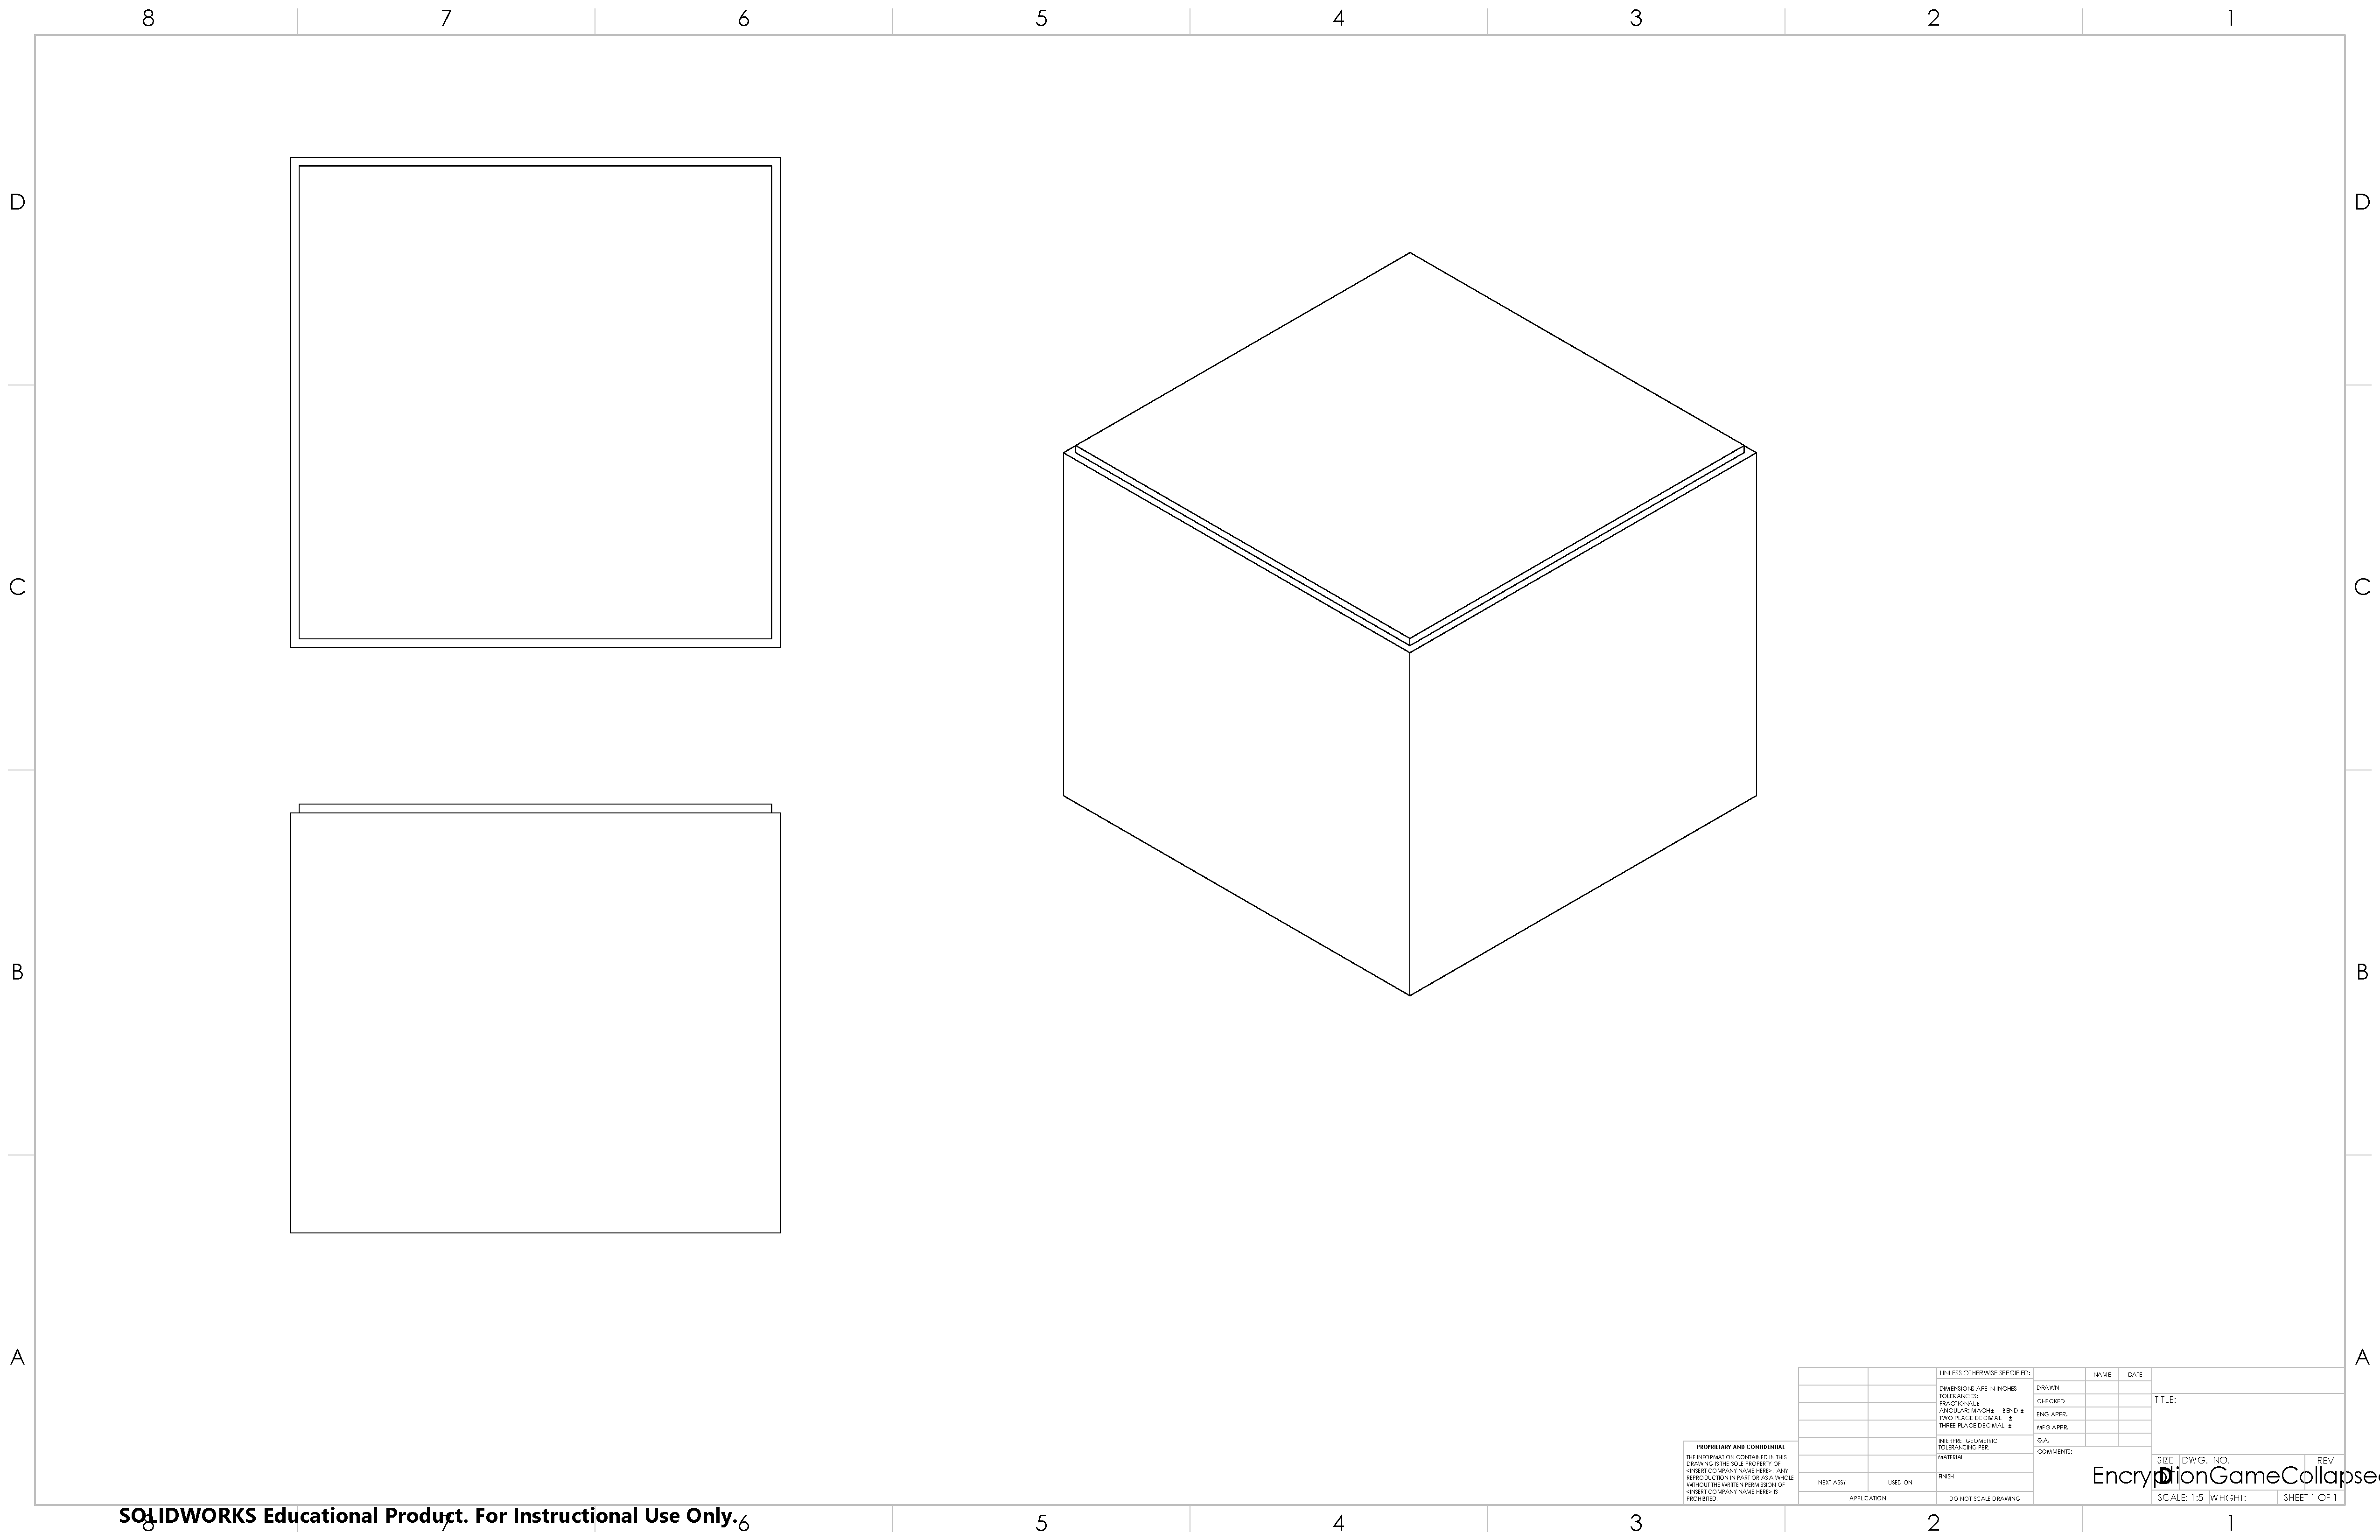
\includepdf[pages=-,angle=90,scale=.95]{Figures/EncryptionGameCollapsed.pdf}
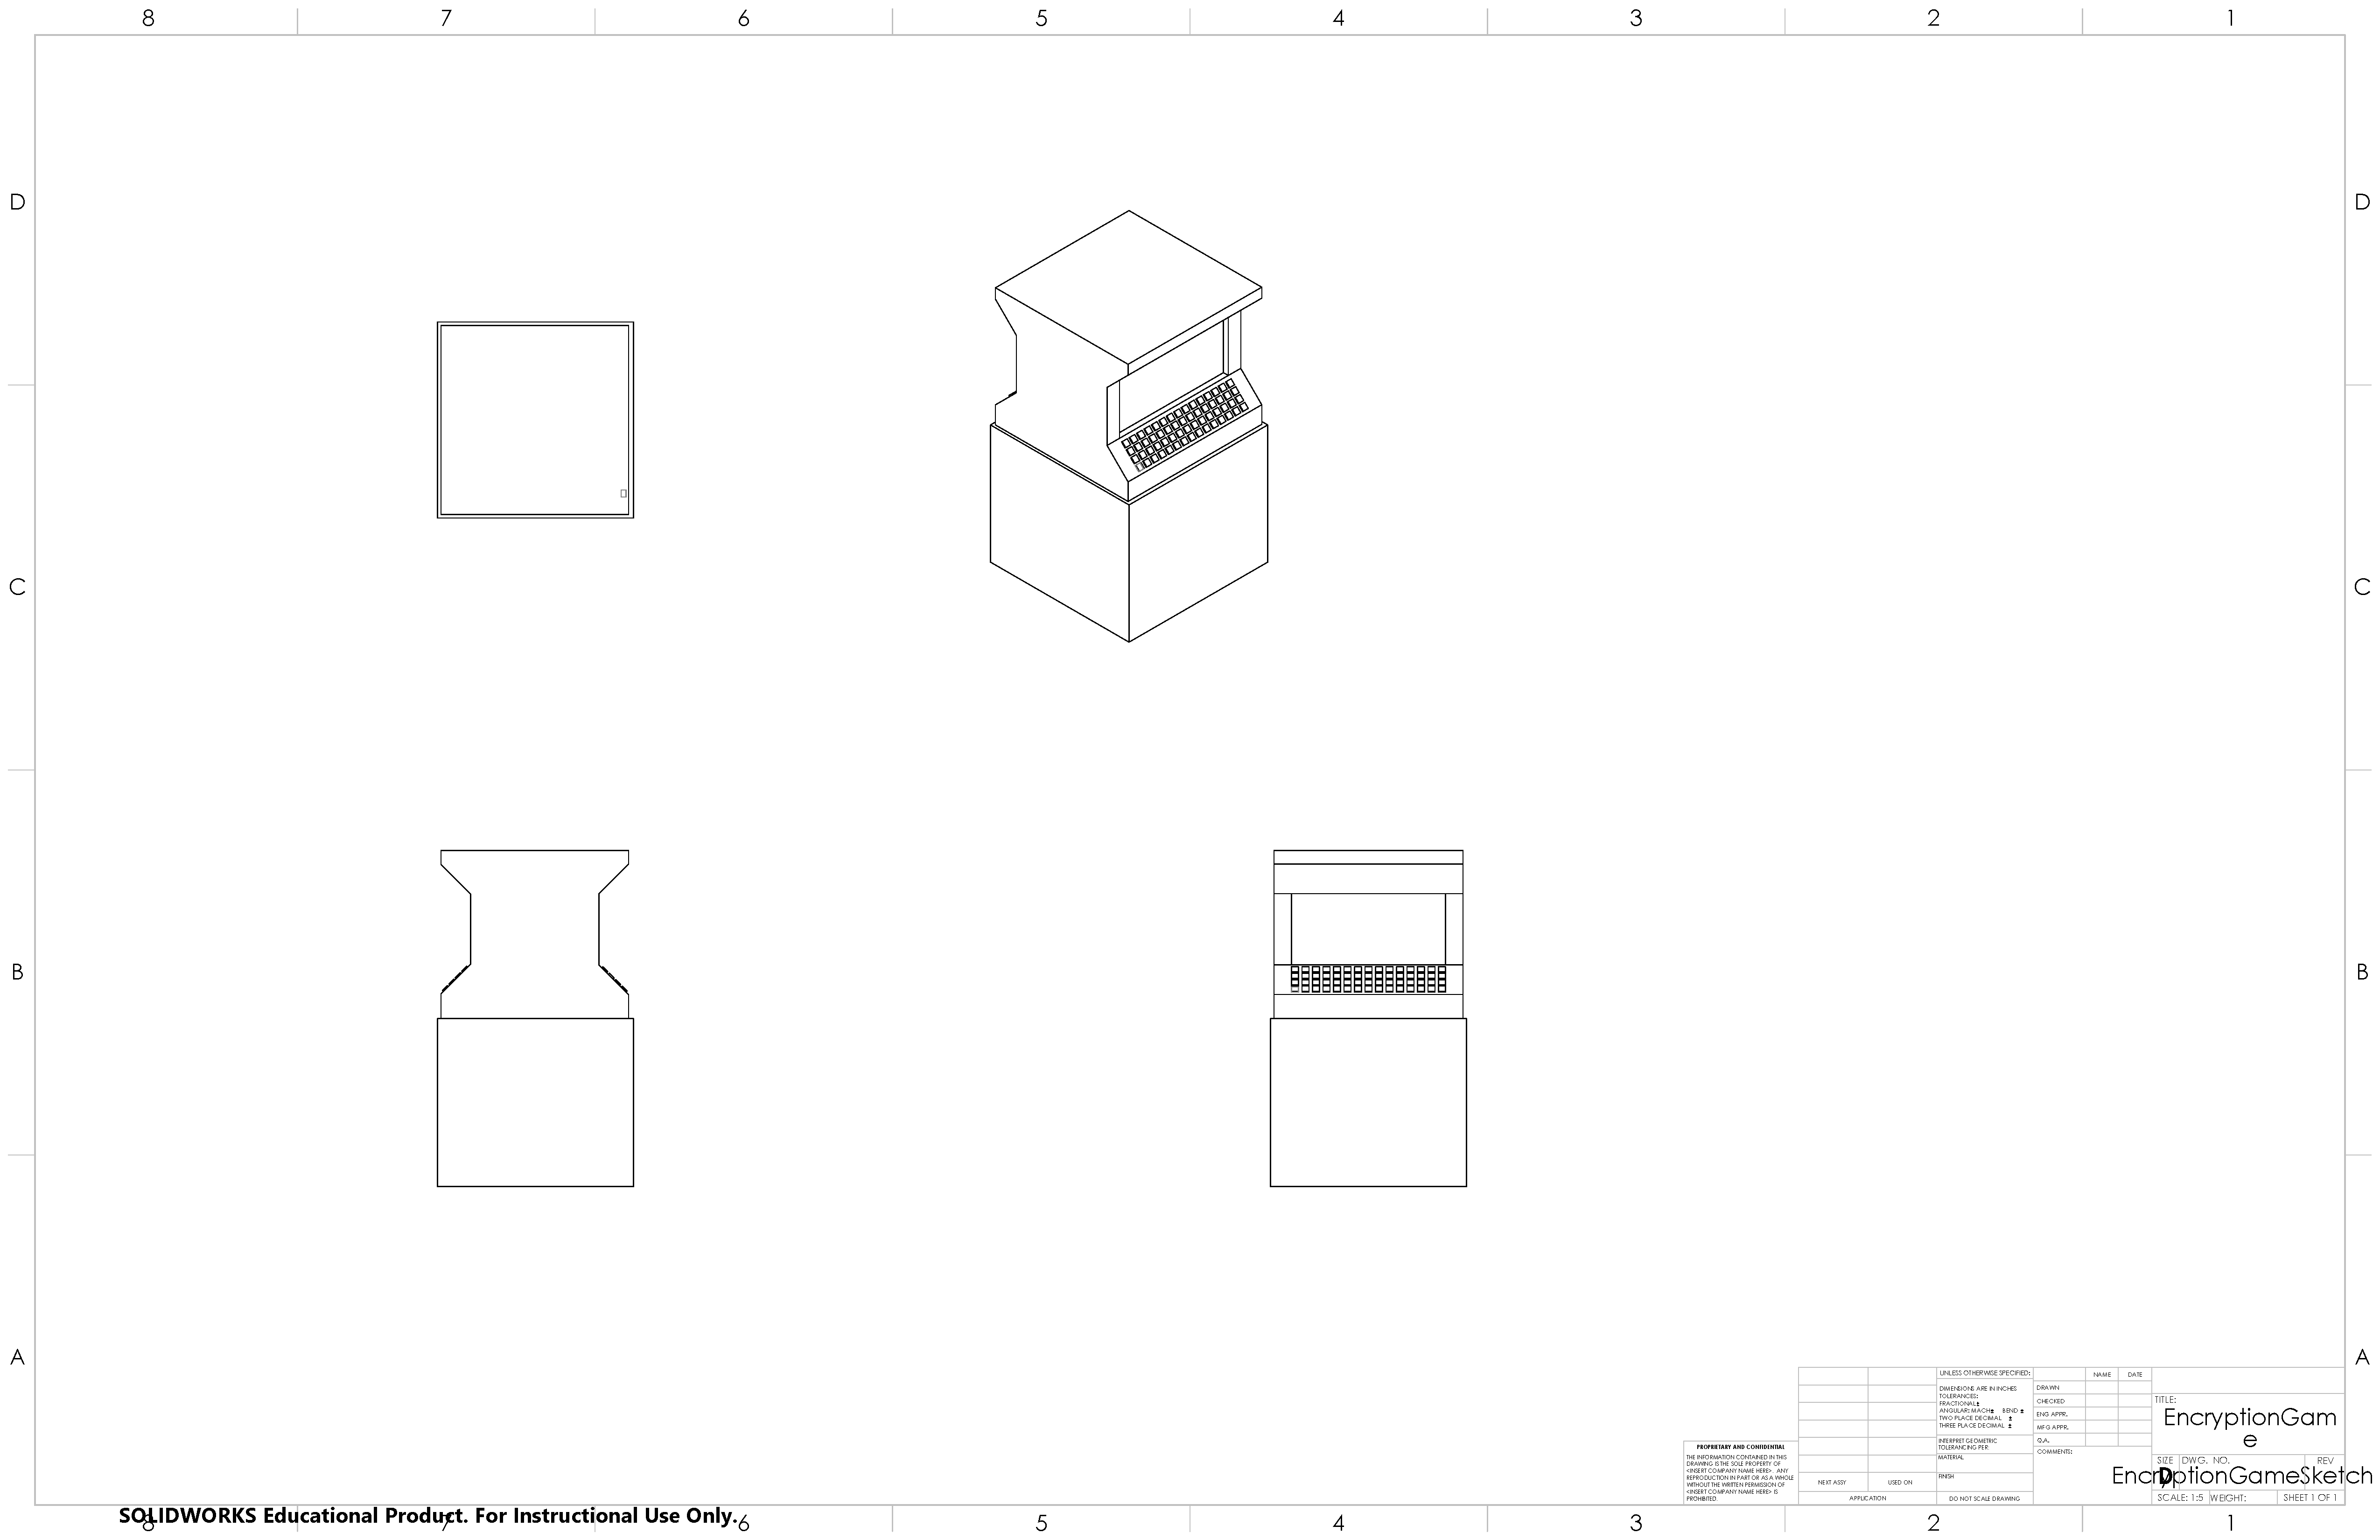
\includepdf[pages=-,angle=90,scale=.95]{Figures/EncryptionGameSketch.pdf}

\addcontentsline{toc}{subsection}{Appendix D — Product Testing Results}

 \hspace{.5in}   \textbf{APPENDIX D — PRODUCT TESTING RESULTS}  

 \vspace{10pt}

\par When looking at preliminary testing, the amount of data actually collected was very minimal. The code for the design was very complex and the majority of the time leading up to the exhibition was spent finalizing it. However, some data points were collected before the exhibit and they heavily contributed to the design’s final functionality. Originally, the design would display a range to the users of how many digits the ASCII values were rotated by. However, by looking at the first few results in appendix K, it is seen that less than ⅓ of users solved the puzzle and those that did had simple encryption phrases and a lot of allotted time. For example, one of the users spent over a minute decrypting the word “tree” (appendix K). 
\par Because of the clear level of difficulty, a decision was made to display the exact number of rotation rather than a range. Immediately there was a clear level of improvement in user success, even going as far as a 9 character phrase being decrypted in 11 seconds. This initial oversight is likely a result of a lack of original testing due to the difficulties finalizing the code. Certain opportunities for data, like the in-class exhibition, were not capitalized on. 
\par For analytical reference, our code also documents the inputted phrase, what it was encrypted, and the number of digits the ASCII value reversed by. This allows for the comparison of phrases of similar length, of similar digit rotation, or both. 

 \newpage

\addcontentsline{toc}{subsection}{Appendix E — Code Used in Project}

 \hspace{.5in}   \textbf{APPENDIX E — CODE USED IN PROJECT}  

\begin{figure}[h!]
  \caption{Encrypt-Decrypt Code}
\end{figure}
\vspace{-15pt}
\lstinputlisting[
    caption=, % Caption above the listing
	label=lst:L1, % Label for referencing this listing
	language=Octave, % Use Octave functions/syntax highlighting
	frame=single, % Frame around the code listing
	showstringspaces=false, % Don't put marks in string spaces
	numbers=left, % Line numbers on left
	numberstyle=\normalsize, % Line numbers styling
    backgroundcolor=\color{black!5}, % Set background color
    keywordstyle=\color{magenta!80}, % Set keyword color
    commentstyle=\color{blue!80}, % Set comment color
    stringstyle=\color{green!80}, % Set string color
    breaklines=true
  ]{Supplements/EncryptionDemo.m}

\begin{figure}[h!]
  \caption{LCD Add-on Code for MATLAB}
\end{figure}
\vspace{-15pt}
\lstinputlisting[
    caption=, % Caption above the listing
	label=lst:L1, % Label for referencing this listing
	language=Octave, % Use Octave functions/syntax highlighting
	frame=single, % Frame around the code listing
	showstringspaces=false, % Don't put marks in string spaces
	numbers=left, % Line numbers on left
	numberstyle=\normalsize, % Line numbers styling
    backgroundcolor=\color{black!5}, % Set background color
    keywordstyle=\color{magenta!80}, % Set keyword color
    commentstyle=\color{blue!80}, % Set comment color
    stringstyle=\color{green!80}, % Set string color
    breaklines=true
  ]{Supplements/LCDAddon.m}

\newpage

\addcontentsline{toc}{subsection}{Appendix F — Wire Diagrams for Sparkfun Board}

 \hspace{.5in}   \textbf{APPENDIX F — WIRE DIAGRAMS FOR SPARKFUN BOARDS}  

 \begin{figure}[H]
   \centering
   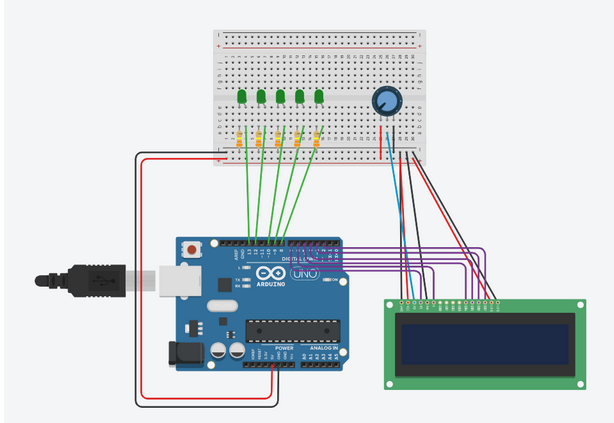
\includegraphics[width=.9\textwidth]{Figures/WireDiagram1.png}
   \caption{Diagram of Circuitry}
   \label{fig:3}
 \end{figure}

 \newpage

\addcontentsline{toc}{subsection}{Appendix G — Photo Log}

 \hspace{.5in}   \textbf{APPENDIX G — PHOTO LOG}  

 \begin{figure}[H]
   \centering
   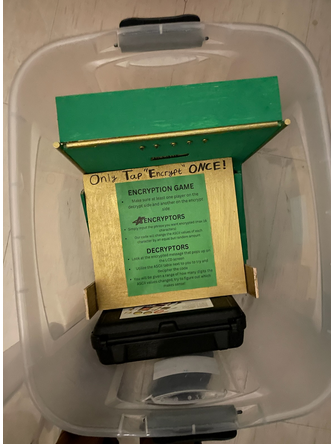
\includegraphics[width=.9\textwidth]{Figures/Log/PhotoLog1.png}
   \caption{Shows Unit in Transportation Mode}
 \end{figure}
 \begin{figure}[H]
   \centering
   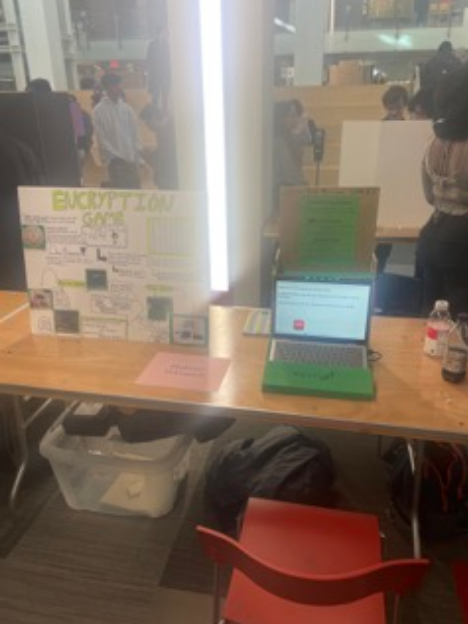
\includegraphics[width=.9\textwidth]{Figures/Log/PhotoLog2.png}
   \caption{Shows Unit Fully Set Up}
 \end{figure}
 \begin{figure}[H]
   \centering
   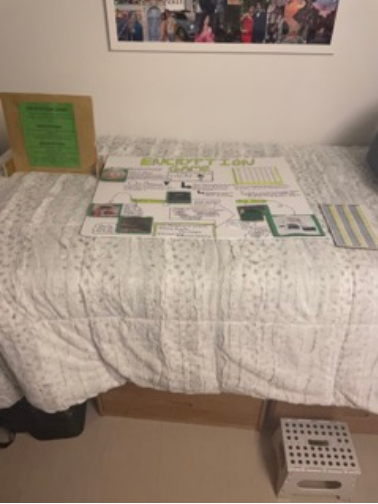
\includegraphics[width=.9\textwidth]{Figures/Log/PhotoLog3.png}
   \caption{Shows Unit Placed in a Team Member's Room}
 \end{figure}
 \begin{figure}[H]
   \centering
   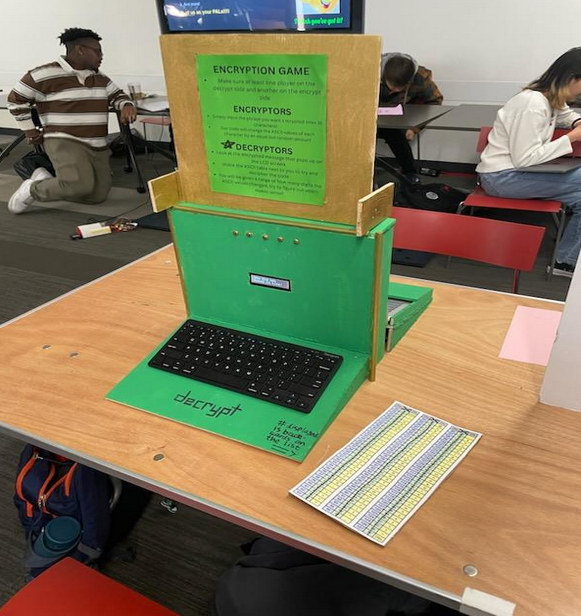
\includegraphics[width=.9\textwidth]{Figures/Log/PhotoLog4.png}
   \caption{Shows Interactive Components of Unit}
 \end{figure}
 \begin{figure}[H]
   \centering
   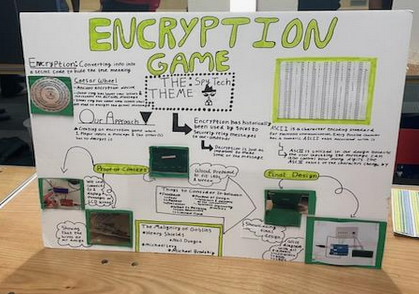
\includegraphics[width=.75\textwidth]{Figures/Log/PhotoLog5.png}
   \caption{Shows Educational Exhibit}
 \end{figure}
 \begin{figure}[H]
   \centering
   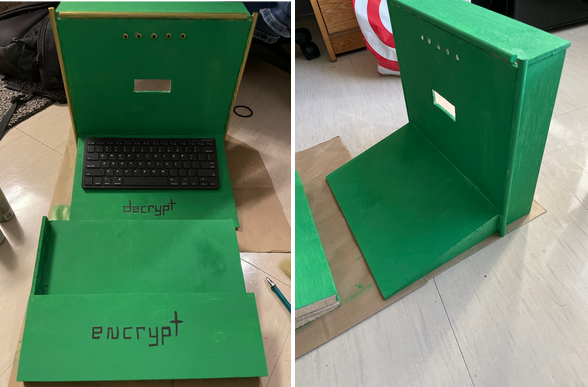
\includegraphics[width=.9\textwidth]{Figures/Log/PhotoLog6.png}
   \caption{Shows Unit at 80\% Completion}
 \end{figure}
 \begin{figure}[H]
   \centering
   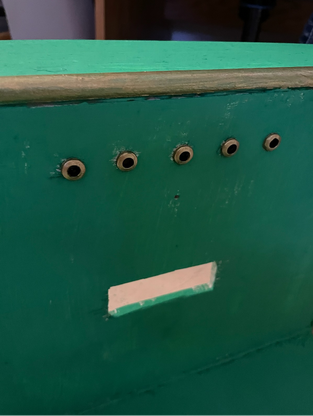
\includegraphics[width=.9\textwidth]{Figures/Log/PhotoLog7.png}
   \caption{Shows LED Components}
 \end{figure}
 \begin{figure}[H]
   \centering
   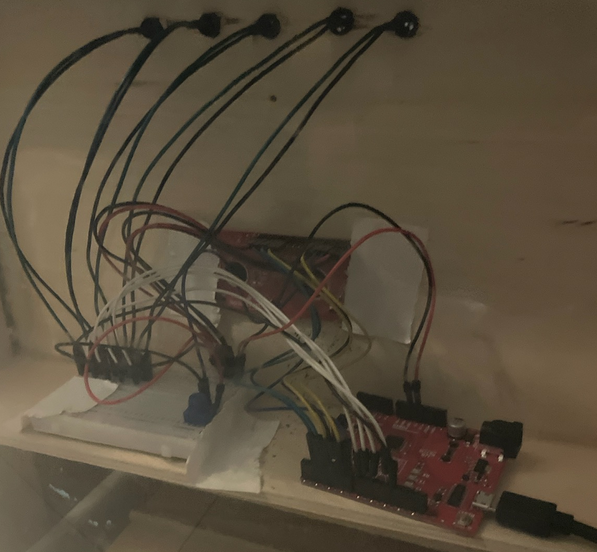
\includegraphics[width=.75\textwidth]{Figures/Log/PhotoLog8.png}
   \caption{Shows Wiring Behind the Unit}
 \end{figure}

\newpage

\addcontentsline{toc}{subsection}{Appendix H — Final Gantt Chart} \label{GC}

 \hspace{.5in}   \textbf{APPENDIX H — FINAL GANTT CHART}  
 \normalsize (See next page) \Large

 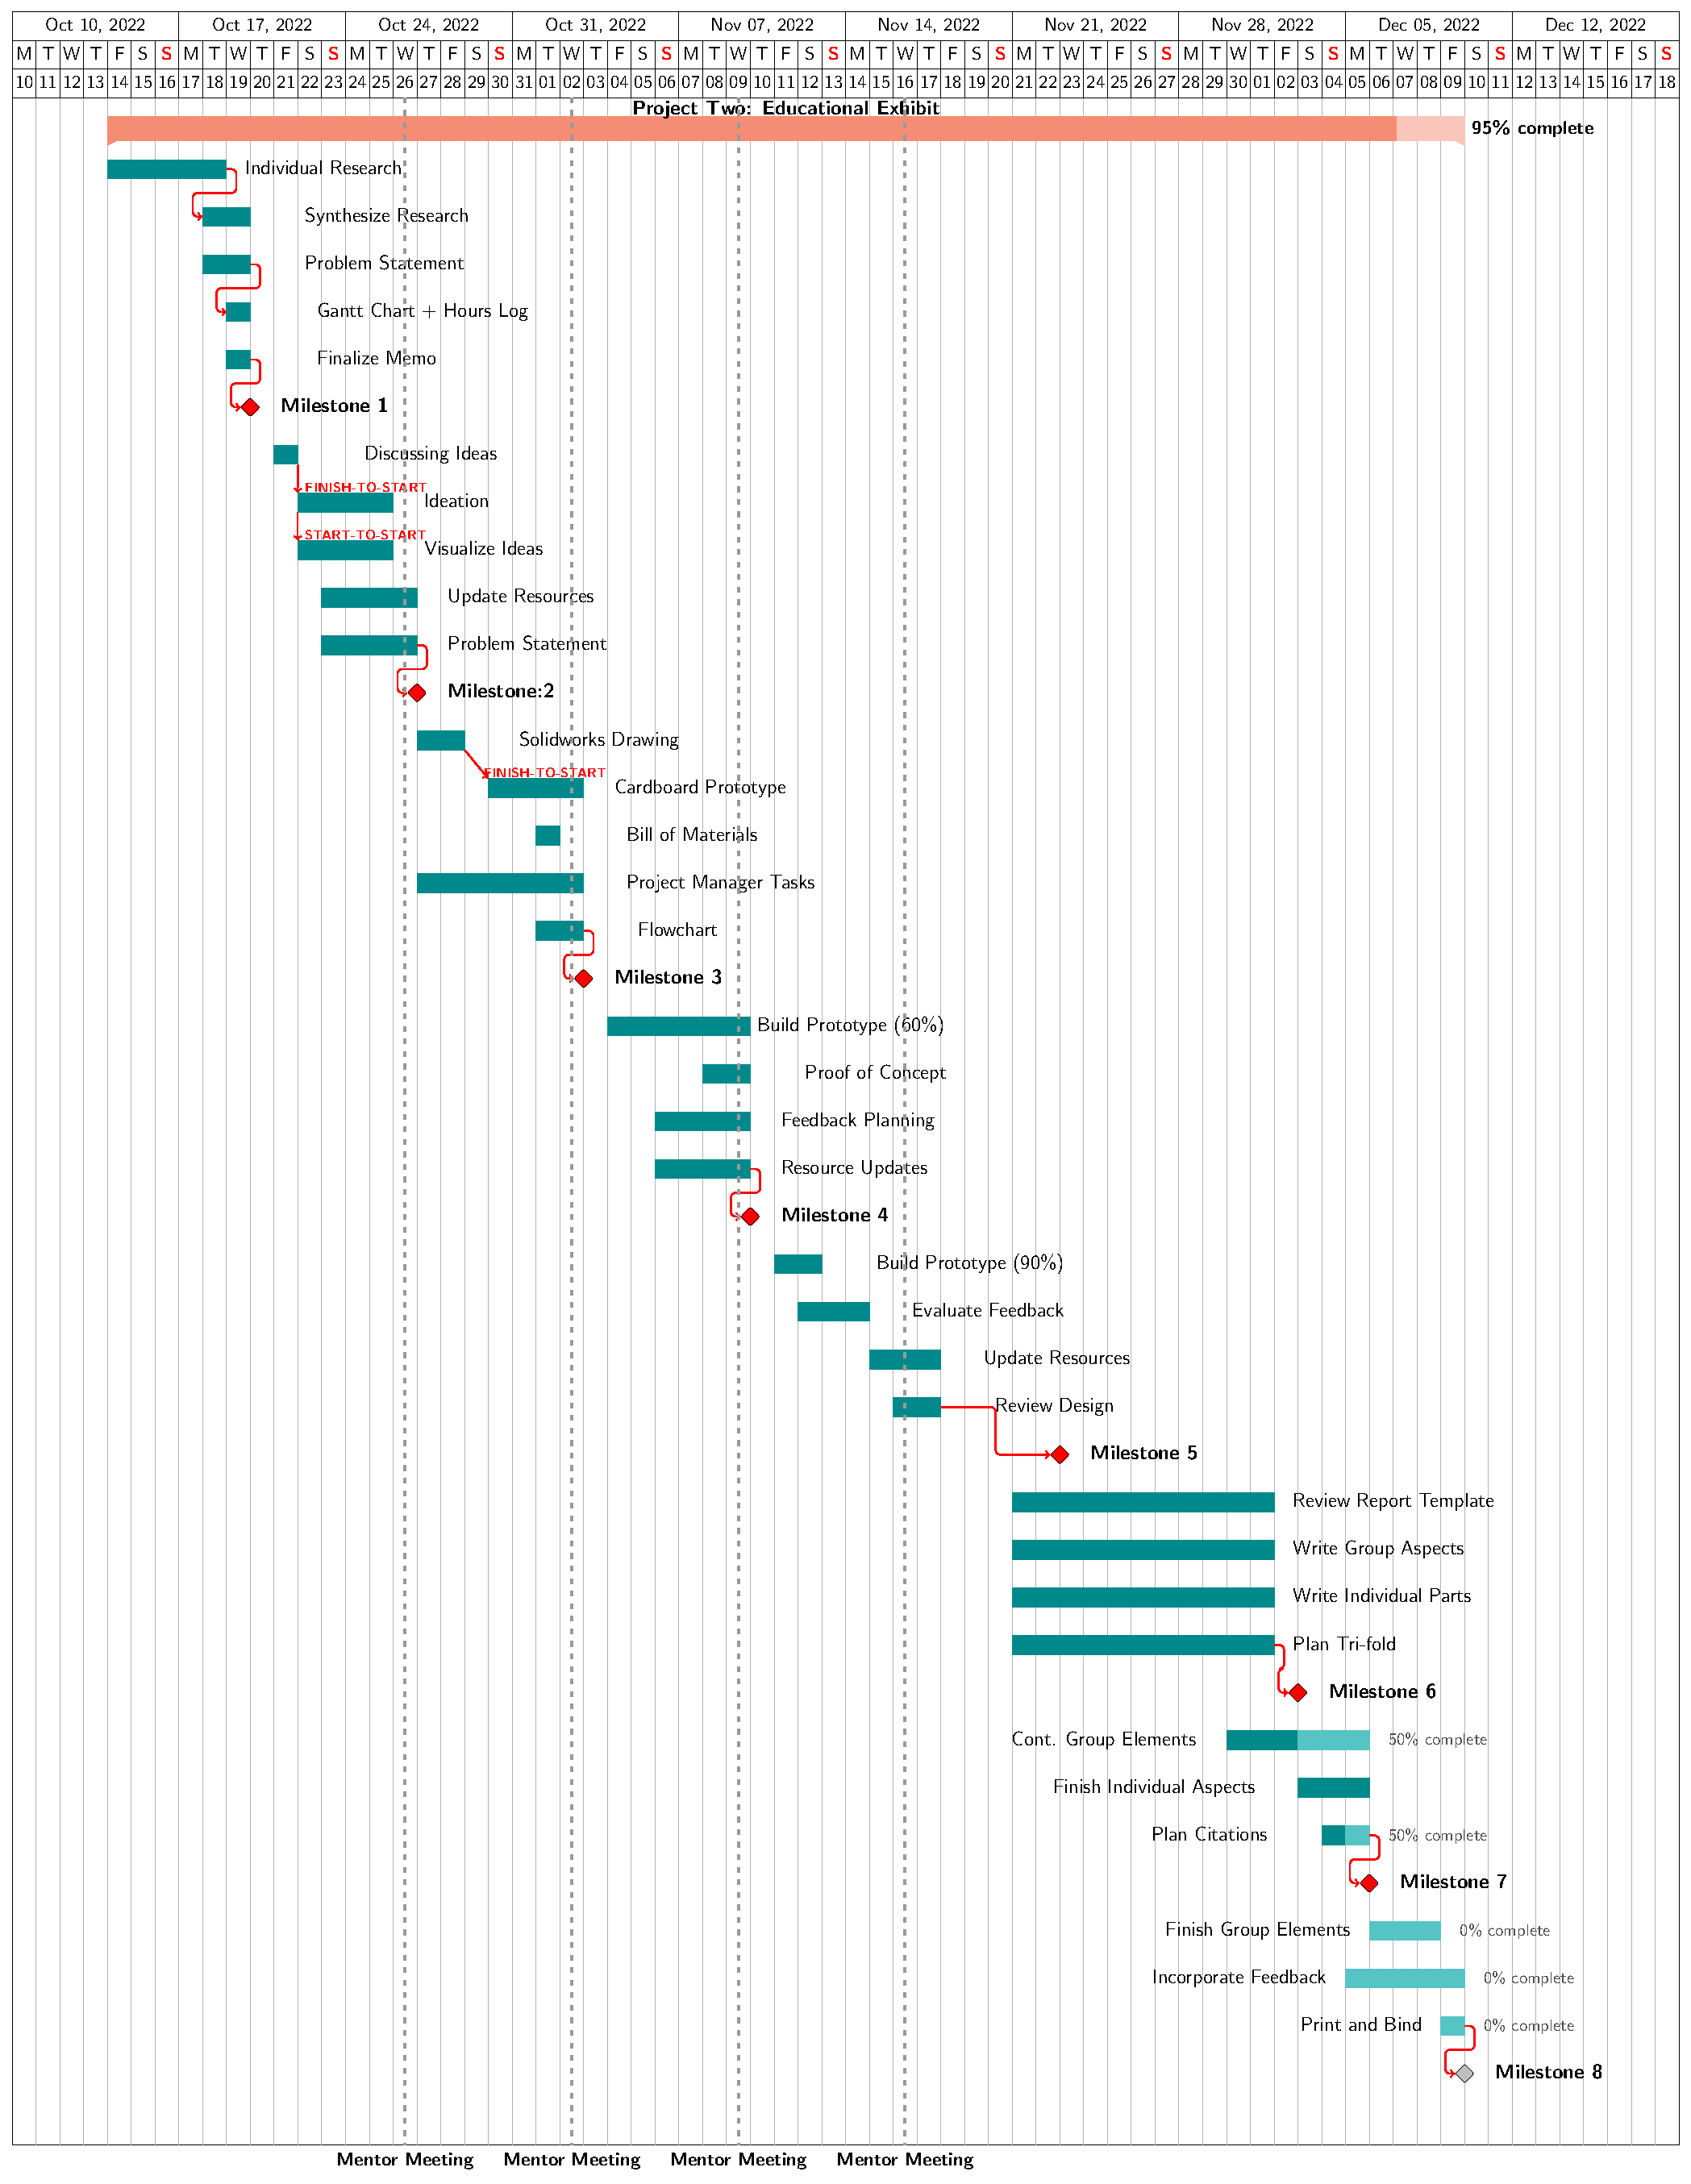
\includepdf[pages=-,scale=.95]{Figures/Gantt.pdf}

 \newpage

\addcontentsline{toc}{subsection}{Appendix I — Final Budget}

 \hspace{.5in}   \textbf{APPENDIX I — FINAL BUDGET}  

   \begin{table}[H]
     \centering
     \begin{tabular}{| l | l | l | l | l | l | l | l |}
       \hline
       \rowcolor{black}\textcolor{white}{Item} & \textcolor{white}{Unit Value} & \textcolor{white}{Units} & \textcolor{white}{Qty} & \textcolor{white}{Value} & \textcolor{white}{Cost} & \textcolor{white}{Source} & \textcolor{white}{Notes}\\
       \hline
       $\nicefrac{3}{8}$'' Dowel & \$.2958 & Dowel & 3 & \$.8874 & \$0 & FYELIC & Used for display-side support\\
       \hline
       \rowcolor{lightgray} $12\times24$'' Plywood & \$10.98 & Sheet & 4 & \$43.92 & \$46.67 & Bookstore & Used for structure \\
       \hline
       $2\times16$ LCD Display & \$8.99 & ea & 1 & \$8.99 & \$0 & Inventor's Kit & Used to display text\\
       \hline
       \rowcolor{lightgray} Arduino Uno & \$28.50 & ea & 1 & \$28.50 & \$0 &Inventor's Kit & Used as a central processor for the system\\
       \hline
       Breadboard & \$9.79 & ea & 1 & \$9.79 & \$0 & Inventor's Kit & Used to connect system more easily\\
       \hline
       \rowcolor{lightgray} Wires & \$.06 & ea & 11 & \$.66 & \$0 & Inventor's Kit & Used to integrate components\\
       \hline
       Potentiometer & \$.89 & ea & 1 & \$.89 & \$0 & Inventor's Kit & Used to control display brightness\\
       \hline
       \rowcolor{lightgray} Wireless Keyboard & \$18.73 & ea & 1 & \$18.73 & \$19.90 & Bookstore & For the user to enter text\\
       \hline
       Paint (Green) & \$4.99 & ea & 2 & \$9.98 & \downarrow & Hardware store & To decorate the device\\
       \hline
       \rowcolor{lightgray} Paint (Gold) & \$5.99 & ea & 1 & \$5.99 & \downarrow & Hardware store & To decorate the device\\
       \hline
       Paintbrush & \$1.99 & ea & 1 & \$1.99 & \downarrow & Hardware store & To use the paint\\
       \hline
       \rowcolor{lightgray} Art Supply Total & \cellcolor{black} & \cellcolor{black} & \cellcolor{black} & \cellcolor{black} & \$19.19 & Hardware store  & Totals above three costs\\
       \hline
     \end{tabular}
     \caption{Final Budget}
     \label{table:4}
   \end{table}

   \newpage

\addcontentsline{toc}{subsection}{Appendix J — Project Hours Log}

 \hspace{.5in}   \textbf{APPENDIX J — PROJECT HOURS LOG}  

 \newpage

\addcontentsline{toc}{subsection}{Appendix K — User Data}

 \hspace{.5 in} \textbf{APPENDIX K — USER DATA}

\vspace{5pt}

\begin{figure}[h!]
  \caption{Collected User Data}
  \label{fig:4}
\end{figure}
\vspace{-15pt}
\lstinputlisting[
    caption=, % Caption above the listing
	label=lst:L1, % Label for referencing this listing
	language=text, 
	frame=single, % Frame around the code listing
	showstringspaces=false, % Don't put marks in string spaces
	numbers=left, % Line numbers on left
	numberstyle=\tiny, % Line numbers styling
    backgroundcolor=\color{black!5}, % Set background color
    keywordstyle=\color{magenta!80}, % Set keyword color
    commentstyle=\color{blue!80}, % Set comment color
    stringstyle=\color{green!80} % Set string color
  ]{Figures/userData.txt}

\end{document}
